%%%%%%%%%%%%%%%%%%%%%%% file template.tex %%%%%%%%%%%%%%%%%%%%%%%%%
%
% This is a general template file for the LaTeX package SVJour3
% for Springer journals.          Springer Heidelberg 2010/09/16
%
% Copy it to a new file with a new name and use it as the basis
% for your article. Delete % signs as needed.
%
% This template includes a few options for different layouts and
% content for various journals. Please consult a previous issue of
% your journal as needed.
%
%%%%%%%%%%%%%%%%%%%%%%%%%%%%%%%%%%%%%%%%%%%%%%%%%%%%%%%%%%%%%%%%%%%
%
% First comes an example EPS file -- just ignore it and
% proceed on the \documentclass line
% your LaTeX will extract the file if required
% \begin{filecontents*}{example.eps}
%!PS-Adobe-3.0 EPSF-3.0
%%BoundingBox: 19 19 221 221
%%CreationDate: Mon Sep 29 1997
%%Creator: programmed by hand (JK)
%%EndComments
% gsave
% newpath
%   20 20 moveto
%   20 220 lineto
%   220 220 lineto
%   220 20 lineto
% closepath
% 2 setlinewidth
% gsave
%   .4 setgray fill
% grestore
% stroke
% grestore
% \end{filecontents*}
%

\RequirePackage{fix-cm}
%
\documentclass[smallextended]{svjour3}       % onecolumn (second format)
%\documentclass{article}
%
\smartqed         % flush right qed marks, e.g. at end of proof




%
\usepackage{mathptmx}      % use Times fonts if available on your TeX system
%


% insert here the call for the packages your document requires
%%% PACKAGES %%%%%%%%%%%%%%%%%%%%%%%%%%%%%%%%%%%%%%%%%%%%%%%%%%%%%%%%%%%%%%%%%%%
\usepackage{amsmath}
%\usepackage{amsthm}
\usepackage{authblk}
\usepackage{caption}
\usepackage{charter}
\usepackage[noadjust]{cite}
\usepackage{enumitem}
\usepackage[letterpaper,margin=1in]{geometry}
\usepackage{graphicx}
\usepackage{ifthen}
\usepackage{bold-extra}
\usepackage[charter]{mathdesign}
%\usepackage{subcaption}

%
% please place your own definitions here and don't use \def but
% \newcommand{}{}
%%% MACROS %%%%%%%%%%%%%%%%%%%%%%%%%%%%%%%%%%%%%%%%%%%%%%%%%%%%%%%%%%%%%%%%%%%%%



%---[ A macro for typesetting "et al." in references ]--------------------------
\newcommand{\etal}{\emph{et~al.}}

%---[ Parenthesization ]----------------------------------------------

\newcommand{\newparentheses}[3]{%
  \expandafter\newcommand\csname #1\endcsname[1]{#2##1#3}%
  \expandafter\newcommand\csname #1L\endcsname[1]{\bigl#2##1\bigr#3}%
  \expandafter\newcommand\csname #1XL\endcsname[1]{\Bigl#2##1\Bigr#3}%
  \expandafter\newcommand\csname #1V\endcsname[1]{\left#2##1\right#3}}

\newparentheses{parens}{(}{)}
\newparentheses{braces}{\{}{\}}
\newparentheses{brackets}{[}{]}
\newparentheses{floor}{\lfloor}{\rfloor}
\newparentheses{ceil}{\lceil}{\rceil}
\newparentheses{abs}{|}{|}
\newparentheses{set}{\{}{\}}
\newparentheses{size}{|}{|}
\newparentheses{seq}{\langle}{\rangle}

%---[ Attributes ]----------------------------------------------------

\makeatletter
\newcommand{\onenewattribute}[4]{%
  \@ifundefined{#2}{\let\@@def\newcommand}{\let\@@def\renewcommand}%
  \expandafter\@@def\csname #2\endcsname[1][]{%
    \def\first@arg{##1}\csname @#2\endcsname}%
  \@ifundefined{@#2}{\let\@@def\newcommand}{\let\@@def\renewcommand}%
  \expandafter\@@def\csname @#2\endcsname[2][]{%
    \ifthenelse{\equal{#1}{sub}}%
    {\csname @@#2\endcsname{##1}{\first@arg}{##2}}%
    {\csname @@#2\endcsname{\first@arg}{##1}{##2}}}
  \@ifundefined{@@#2}{\let\@@def\newcommand}{\let\@@def\renewcommand}%
  \expandafter\@@def\csname @@#2\endcsname[3]{%
    \ifthenelse{\equal{##1}{}}%
    {\ifthenelse{\equal{##2}{}}%
      {#3\csname #4\endcsname{##3}}%
      {#3_{##2}\csname #4\endcsname{##3}}}%
    {\ifthenelse{\equal{##2}{}}%
      {#3^{##1}\csname #4\endcsname{##3}}%
      {#3_{##2}^{##1}\csname #4\endcsname{##3}}}}}
\newcommand{\newattribute}[3][sub]{%
  \onenewattribute{#1}{#2}{#3}{parens}%
  \onenewattribute{#1}{#2L}{#3}{parensL}%
  \onenewattribute{#1}{#2XL}{#3}{parensXL}%
  \onenewattribute{#1}{#2V}{#3}{parensV}}

\newcommand{\newproperty}[2]{%
  \@ifundefined{#1}{\let\@@def\newcommand}{\let\@@def\renewcommand}%
  \expandafter\@@def\csname #1\endcsname[1][]{%
    {\ifthenelse{\equal{##1}{}}%
      {#2}%
      {#2_{##1}}}}}

\makeatother

%---[ Asymptotic notation ]-------------------------------------------

\newattribute{OhOf}{\mathrm{O}}
\newattribute{ThetaOf}{\Theta}
\newattribute{OmegaOf}{\Omega}
\newattribute{ohOf}{\mathrm{o}}
\newattribute{omegaOf}{\omega}

\newcommand{\BigOh}[1]{O\!\left(#1\right)}
\newcommand{\LittleOh}[1]{o\!\left(#1\right)}

%---[ Macros for a bunch of operations we perform ]-----------------------------

\newcommand{\rankopsym}{\texttt{rank}}
\newattribute{rankop}{\rankopsym}
\newcommand{\selopsym}{\texttt{select}}
\newattribute{selop}{\selopsym}
\newcommand{\stepop}{\texttt{step}}
\newcommand{\regpossym}{\texttt{rpos}}
\newattribute{regpos}{\regpossym}
\newcommand{\subregpossym}{\texttt{spos}}
\newattribute{subregpos}{\subregpossym}
\newcommand{\possubregsym}{\texttt{sreg}}
\newattribute{possubreg}{\possubregsym}
\newcommand{\bdcountsym}{\texttt{sbdcount}}
\newattribute{bdcount}{\bdcountsym}

%---[ Macros for some concepts ]------------------------------------------------

\newcommand{\path}{K}
\newcommand{\pointset}{P}
\newcommand{\reals}{\mathbb{R}}
\newcommand{\plane}{\reals^2}
\newcommand{\triang}{\mathcal{T}}
\newcommand{\dual}[1]{#1^*}
\newcommand{\augdual}[1]{#1^+}

\newattribute{deg}{d}
\newattribute{nb}{N}

\newcommand{\regsz}{r_1}
\newcommand{\subregsz}{r_2}
\newcommand{\regub}{s_R}
\newcommand{\subregub}{s_S}

\newattribute{glbl}{\ell_G}
\newattribute{reglbl}{\ell}
\newattribute{subreglbl}{\ell}

\newproperty{reg}{R}
\newproperty{subreg}{R}
\newproperty{perm}{\pi}
\newproperty{graphrep}{\mathcal{G}}
\newproperty{numv}{n}
\newproperty{dnumv}{n'}
\newproperty{bdvec}{\mathcal{B}}
\newproperty{keyvec}{\mathcal{K}}
\newproperty{lblvec}{\mathcal{L}}
\newproperty{fstofreg}{\mathcal{F}_R}
\newproperty{fstofsubreg}{\mathcal{F}_S}
\newproperty{defvec}{\mathcal{D}}
\newproperty{vvec}{\mathcal{V}}
\newproperty{regvec}{\mathcal{R}}
\newproperty{subregvec}{\mathcal{R}_{\ell} } %was \mathcal{S} S, but clashes with \ds
\newproperty{idxvec}{\mathcal{I}}

\newproperty{term}{\mathcal{T}}
\newproperty{pos}{p}
\newproperty{genvec}{\mathcal{A}}

\newcommand{\ds}{\mathcal{S}}
\newcommand{\fst}{\mathcal{F}}
\newcommand{\diff}{\mathcal{D}}
\newcommand{\regnbvec}{\mathcal{N}_R}
\newcommand{\subregnbvec}{\mathcal{N}_S}
\newcommand{\regminvec}{\mathcal{M}_R}
\newcommand{\subregminvec}{\mathcal{M}_S}
\newcommand{\regbdvec}{\bdvec[R]}
\newcommand{\subregbdvec}{\bdvec[S]}
\newcommand{\reglt}{\prec_R}
\newcommand{\subreglt}{\prec_S}
%\newcommand{\succblksize}{\textbf{\textsc{B}}}
\newcommand{\succblksize}{\textbf{b}}

\newcommand{\regptable}{\mathcal{P}_R}
\newcommand{\subregptable}{\mathcal{P}_{SR}}



\newcommand{\wsize}{w}
\newcommand{\augdualsym}{+}
\newcommand{\concomp}{{\triang}_C}
\newcommand{\bitsPerKey}{q}
\newcommand{\bitsPerPoint}{\phi}
\newcommand{\funccase}[1]{\texttt{#1}}

%---[ Caligraphic letters to be replaced by mnemonics later ]-------------------

\newcommand{\B}{\mathcal{B}}
\newcommand{\D}{\mathcal{D}}
\newcommand{\F}{\mathcal{F}}
\newcommand{\G}{\mathcal{G}}
\newcommand{\K}{\mathcal{K}}
\renewcommand{\L}{\mathcal{L}}
\newcommand{\N}{\mathcal{N}}
\renewcommand{\S}{\mathcal{S}}
\newcommand{\T}{\mathcal{T}}

%---[ Two dots for typesetting ranges ]-----------------------------------------

\newcommand{\tdots}{\mathinner{\ldotp\ldotp}}

%---[ Some beautification ]-----------------------------------------------------

\let\epsilon\varepsilon

%
% Insert the name of "your journal" with
\journalname{Algorithmica}
%
\begin{document}

\title{I/O-Efficient Path Traversal in Succinct Planar Graphs}
%\subtitle{Do you have a subtitle?\\ If so, write it here}

%\titlerunning{Short form of title}        % if too long for running head

\author{Craig Dillabaugh         \and
        Meng He \and
        Anil Maheshwari \and
        Norbert Zeh
}

%\authorrunning{Short form of author list} % if too long for running head

\institute{Craig Dillabaugh \at
              School of Computer Science, Carleton University \\
              Tel.: +819-827-8215\\
              Fax:  +613-520-4334\\
              \email{cdillaba@cg.scs.carleton.ca}           %  \\
%             \emph{Present address:} of F. Author  %  if needed
           \and
           Meng He \at
           Faculty of Computer Science, Dalhousie University \\
	   6050 University Avenue, PO BOX 15000, Halifax, NS B3H 4R2, Canada
           \and
           Anil Maheshwari \at
           School of Computer Science,  Carleton University \\
           5302 HP, 1125 Colonel By Drive, Ottawa, ON K1S 5B6, Canada
           \and
           Norbert Zeh \at
           Faculty of Computer Science, Dalhousie University \\
	   6050 University Ave, Halifax, NS B3H 1W5, Canada
}

\date{Received: date / Accepted: date}
% The correct dates will be entered by the editor


\maketitle

\begin{abstract}

  We present a technique for representing bounded-degree planar graphs
  in a succinct fashion while permitting I/O-efficient traversal of
  paths.
  Using our representation, a graph with $N$ vertices, each
  with an associated key of $\bitsPerKey = \OhOf{\lg N}$ bits,\footnote{In this
    paper $\lg{N}$ denotes $\log_2{N}$.} can be stored in $N\bitsPerKey
  + \OhOf{N} + \ohOf{N\bitsPerKey}$ bits and traversing a path of length $K$ 
  takes $\OhOf{K
  / \lg B}$ I/Os, where $B$ denotes the disk block size.
  By applying our construction to the dual of a terrain represented as a
  triangular irregular network, we can represent the terrain in the
  above space bounds and support path traversals on the terrain using
  $\OhOf{K / \lg B}$ I/Os, where $K$ is the number of triangles visited by
  the path.
  This is useful for answering a number of queries on the
  terrain, such as reporting terrain profiles, trickle paths, and
  connected components.

\keywords{external memory algorithms \and path traversal \and 
planar graphs \and succinct data structures }
% \PACS{PACS code1 \and PACS code2 \and more}
% \subclass{MSC code1 \and MSC code2 \and more}
\end{abstract}


% ------------------------------------------------------------------------------
\section{Introduction}
% ------------------------------------------------------------------------------

External memory (EM) data structures and succinct data structures both
address the problem of representing very large data sets.
In the EM model, the goal is to structure data that are too large to fit into
internal memory in a way that minimizes the transfer of data between
internal and external memory when answering certain queries.
For succinct data structures, the aim is to encode the structural
component of the data structure using as little space as is
theoretically possible while still permitting efficient navigation of
the structure.
Thus, EM data structures deal with the I/O bottleneck
that arises when the data are too large to fit into memory, while
succinct data structures help to avoid this bottleneck as they allow
more data to be stored in memory.
Succinct EM data structures maximize the amount of data that fits on a disk of
a given size or in a disk block.
The former is important because an increasing number of
large-scale applications find themselves limited by the amount of data
that fits on a disk.
The latter helps to reduce the I/O bottleneck further, as more useful data
can be swapped between memory and disk in a single I/O operation.

In this paper, we develop a succinct EM data structure for path
traversal in planar graphs.
Given a bounded-degree planar graph $G$,
our goal is to simultaneously minimize the amount of space used to
store $G$ on disk as well as the number of I/O operations required to report
a path of length $K$ in $G$.
As practical applications of our
structure, we show how it can be used to answer a range of important
queries on triangular irregular network (TIN) models of terrains.

% ------------------------------------------------------------------------------
\subsection{Background}\label{sec:background}
% ------------------------------------------------------------------------------

In the \emph{external memory} (EM) model \cite{DBLP:journals/cacm/AggarwalV88}, the
computer is assumed to be equipped with a two-level memory hierarchy
consisting of \emph{internal} and (disk-based) \emph{external memory}.
The external memory is assumed to have infinite size, but accessing data
elements in external memory is several orders of magnitude slower than accessing
data in internal memory.
Conversely, while internal memory permits efficient operations, its size is limited
to $M$ data elements.
Data is transferred between internal and external memory by means of
\emph{I/O operations} (\emph{I/Os} for short), each of which transfers
a block of $B$ consecutive data items. 
The efficiency of a data structure in the EM model is measured in terms of the
space it uses and the number of I/Os required to answer certain queries.
In order to take advantage of blockwise disk accesses, it is necessary that $M
\ge B$.
In this paper, we assume $M \ge 2B$ and $B = \OmegaOf{\lg N}$,
where $N$ denotes the input size. Furthermore, we assume that the machine
word size is $\wsize = \Theta(\lg N)$ bits, an assumption commonly used 
in papers on succinct data structures in internal 
memory~\cite{DBLP:journals/talg/RamanRS07}.

Nodine~\etal~\cite{ngv_1996} first explored the problem of blocking
graphs in external memory for efficient path traversal. They store the
 graph in disk blocks (possibly with duplication of
vertices and edges) so that any path in the graph could be traversed
using few I/Os relative to the path's length.
The efficiency of the blocking is expressed in terms
of the \emph{blocking speed-up}, which is the minimum ratio between
the length of a traversed path and the number of I/Os required to
traverse it, taken over all paths that require more than $c$ I/Os to
traverse, for some constant $c$, and assuming that only one block can
be held in memory at any point in time.
The authors identified the optimal bounds for the worst-case blocking speed-up
for several classes of graphs.
Agarwal \etal~\cite{DBLP:conf/soda/AgarwalAMVV98} proposed a
blocking of bounded-degree planar graphs such that any path of length
$K$ can be traversed using $\OhOf{K / \lg B}$ I/Os.

Succinct data structures represent their structural
components using space as near the information-theoretic lower bound as
possible while still permitting efficient operations.
These were originally proposed by Jacobson
\cite{jac_1989}, who designed succinct representations of trees and
graphs.
To represent graphs, Jacobson relied on the technique of book
embeddings by Bernhart and Kainen
\cite{DBLP:journals/jct/BernhartK79}.
A $k$-page book embedding of a graph is an ordering of the graph's vertices,
along with a partition of its edges into $k$ ``pages'',
each of which is a subset of edges that induces an outerplanar embedding of
the graph consistent with the chosen vertex ordering.
Yannakakis \cite{DBLP:conf/stoc/Yannakakis86}
demonstrated that $k=4$ is necessary and sufficient to partition
planar graphs.
Jacobson's data structure embeds each page of a graph
on $N$ vertices using $\OhOf{N}$ bits, and can thus represent
$k$-page graphs using $\OhOf{kN}$ bits and planar graphs using
$\OhOf{N}$ bits.
The structure supports adjacency queries using
$\OhOf{\lg N}$ bit probes, and the listing of the neighbours of a
vertex $v$ of degree $\deg{v}$ using $\OhOf{\deg{v} \lg N + k}$ bit
probes.

Jacobson's result was improved upon by Munro and Raman
\cite{DBLP:conf/focs/MunroR97} under the word-RAM model.
They showed how to represent a $k$-page graph with $N$ vertices and $M$ edges
using $2kN + 2M + \ohOf{Nk + M}$ bits such that adjacency and
vertex degree queries can be answered in $\OhOf{k}$ time.
The neighbours of a vertex $v$ can be reported in $\OhOf{d(v)+k}$ time.
For planar graphs, this result translates to an $(8N + 2M + \ohOf{N+M})$-bit
representation that answers adjacency and degree queries in constant
time, and lists neighbours in $\OhOf{\deg{v}}$ time.
Gavoille and Hanusse \cite{DBLP:journals/dmtcs/GavoilleH08} proposed an encoding
for $M$-edge $k$-page-embeddable graphs that allows multiple edges and
loops.
For a graph with no isolated vertices, their structure uses $2M
\lg k + 4M$ bits, which is an improvement over Munro and Raman's
structure whenever $M \le kN / (2\lg k)$.
By adding an auxiliary table of $\ohOf{M \lg k}$ bits, this encoding
supports calculating vertex degrees in constant time, answering adjacency
queries in $\OhOf{\lg k}$ time (constant for planar graphs), and
accessing all neighbours of a vertex in $\OhOf{\deg{v}}$ time.

An alternate approach to book embeddings of planar graphs, which uses
canonical orderings of the graph's vertices and edges, was presented
by Chuang \etal~\cite{chuang_et_al_1998}.
Their solution represents a planar graph using
$2M + (5 + 1/\epsilon)N + \ohOf{M + N}$ bits, for any $\epsilon > 0$ 
(with $\epsilon = \OhOf{1}$), and supports constant-time adjacency 
and degree queries.
If the graph is simple, this bound becomes
$\frac{5}{3}M + (5 + 1/\epsilon)N + \ohOf{N}$. 
For triangulated planar graphs, they reduced the space
bound to $2M + 2N + \ohOf{N}$ bits.
The space bound for general planar graphs was reduced by Chiang
\etal~\cite{DBLP:journals/siamcomp/ChiangLL05}, who showed that a
graph with no multiple edges or self loops can be represented using
$2M + 2N + \ohOf{M + N}$ bits to support the same set of
operations.
For the case of triangulated planar graphs, Yamanaka and
Nakano~\cite{DBLP:conf/walcom/YamanakaN08} presented an encoding that
uses $2N + \ohOf{M}$ bits and supports adjacency, degree, and
clockwise neighbour queries in constant time.

Barbay \etal~\cite{DBLP:conf/isaac/BarbayAHM07} presented several
results with respect to both planar graphs, triangulations, and
$k$-page graphs, including the first results for labeled graphs and
triangulations.
For planar triangulations, they added support for
rank/select queries of edges in counterclockwise order using $2M
\lg 6 + \ohOf{M}$ bits.
For plane graphs, their structures support
standard queries, as well as rank/select queries in counterclockwise
order, using $3N(2 \lg 3 + 3 + \epsilon) + \ohOf{N}$
bits (for $0 < \epsilon < 1$).
For $k$-page graphs
with large values of $k$, they proposed a representation using $N + 2M
\lg k + M \cdot \ohOf{\lg k} + \OhOf{M}$ bits and supporting
adjacency queries in $\OhOf{\lg k \lg\lg k}$ time, degree queries in
constant time, and the listing of neighbours in $\OhOf{\deg{v} \lg\lg k}$ time.
An alternative representation uses
$N + (2 + \epsilon)M \lg k + M \cdot \ohOf{\lg k} + \OhOf{M}$ bits and
supports adjacency queries in $\OhOf{\lg k}$ time, degree queries in
constant time, and the listing of neighbours in $\OhOf{\deg{v}}$ time.

A third strategy for succinct graph representations is based on graph
partitions.
Aleardi \etal~\cite{DBLP:conf/wads/AleardiDS05}
introduced a succinct representation for triangulations with a
boundary based on a hierarchical partition of the triangulation.
The combinatorial structure of the triangulation is partitioned into small
sub-triangulations which are further partitioned into tiny
sub-triangulations.
The representation stores the connectivity
information with asymptotically 2.175 bits per triangle, and supports
navigation between triangles in constant time.
The same authors presented an improved result of 1.62 bits per triangle for
triangulations without a boundary, and also demonstrated that
3-connected planar graphs can be represented with 2 bits per edge
\cite{DBLP:journals/tcs/AleardiDS08}.
For both planar triangulations and 3-connected planar graphs, this
representation permits constant-time navigation using additional
$\OhOf{N \lg \lg N \mathop{/} \lg N}$ bits of storage.
A partitioning approach was also
employed by Blandford \cite{DBLP:conf/soda/BlandfordBK03}, who showed
that graphs with small separators can be represented using $\OhOf{N}$
bits and such that adjacency and degree queries can be answered in
constant time and listing the neighbours of a vertex takes
$\OhOf{\deg{v}}$ time.

Farzan and Munro \cite{DBLP:conf/esa/FarzanM08} considered
the case of succinct representations of arbitrary graphs.
They described an encoding that requires
$(1 + \epsilon) \lg \parensXL{\genfrac{}{}{0pt}{}{N^2}{M}}$ bits,
for an arbitrarily small constant $\epsilon > 0$,
and supports adjacency and degree queries in constant
time, and the listing of neighbours in $\OhOf{\deg{v}}$ time.

Little work has focused on obtaining succinct EM data structures.
The only results of which we are aware focus on text indexing \cite{DBLP:conf/dcc/ChienHSV08,
  clark_96}, and on path traversals in trees \cite{DillabaughHM08}.

% ------------------------------------------------------------------------------
\subsection{Our Contributions}
% ------------------------------------------------------------------------------

In this paper, we present the following results:

\begin{enumerate}
\item In Section \ref{sec:graph_rep}, we present a data structure that
  uses $Nq + \OhOf{N} + \ohOf{Nq}$ bits to represent a bounded degree 
  planar graph with $N$
  vertices, each with a label of size $q$, and which allows the traversal of
  any path of length $K$ using $O(K / \lg B)$ I/Os.
  This path traversal cost matches that achieved by the data structure of
  Agarwal \etal~\cite{DBLP:conf/soda/AgarwalAMVV98}, but the latter
  uses $\ThetaOf{N \lg N} + 2Nq$ bits to store the graph.
  In the context of large datasets, this space saving represents a
  considerable improvement.
  (e.g., with keys of constant size, the space bound improves by
  a factor of $\lg N$.)
\item In Section \ref{sec:tins}, we apply our structure to store
  triangulations.
  If storing a point requires $\bitsPerPoint$ bits, we are able to store a triangulation in
  $N \bitsPerPoint + \OhOf{N} + \ohOf{N \bitsPerPoint}$ bits so that any path crossing $K$
  triangles can be traversed using $\OhOf{K / \lg B}$ I/Os.
  Again, the I/O efficiency of our structure matches that
  of~\cite{DBLP:conf/soda/AgarwalAMVV98} with a similar space improvement
  as for bounded-degree planar graphs.
\item In Section \ref{sec:point_location}, we show how to
  augment our triangulation representation with $\ohOf{N\bitsPerPoint}$ bits of extra
  information in order to support point location 
  queries using $\OhOf{\log_B N}$ I/Os.
  Asymptotically, this does not change the space requirements.
\item In Section \ref{sec:applications}, we describe several
  applications that make use of our representation for triangulations
  from Section~\ref{sec:tins}.
  We demonstrate that reporting terrain profiles and trickle paths takes
  $\BigOh{K / \lg B}$ I/Os.
  We show that connected-component queries---that is, reporting a set of
  triangles that share a common attribute and induce a connected
  subgraph in the triangulation's dual---can be performed using
  $\BigOh{K / \lg B}$ I/Os when the component being reported is convex and consists
  of $K$ triangles.
  For non-convex regions with holes, we achieve a query bound of
  $\BigOh{K / \lg B + h \log_B h}$, where $h$ is the number
  of edges on the component's boundary.
  In order to achieve this query bound, the query procedure uses
  $\BigOh{h \cdot (\bitsPerKey + \lg h)}$ extra space.
  The same query can be answered using no additional space in 
  $\BigOh{K / \lg B + h' \log_B h'}$ I/Os, where $h'$ is the number of
  triangles that are incident on the boundary of the component.
\end{enumerate}


% ------------------------------------------------------------------------------
\section{Preliminaries}
% ------------------------------------------------------------------------------

% ------------------------------------------------------------------------------
\paragraph{Rank and select queries on bit vectors.}
% ------------------------------------------------------------------------------

As is the case for a wide range of succinct data structures, our data
structure relies on succinct representations of bit vectors
that allow constant-time rank and select queries.
Given a bit vector $S[1 \tdots N]$, and a bit value $x \in \{0, 1\}$, a
$\rankop[x]{S, i}$ operation returns the number of $x$s in $S[1 \tdots
i]$, while a $\selop[x]{S, r}$ operation returns the index of the
$r$th $x$ in~$S$.
In other words, $\selop[x]{S, r} = \min \set{i \mid \rankop[x]{S, i} = r}$.
The problem of representing a bit vector succinctly to support
$\rankopsym$ and $\selopsym$ operations in constant time in the word RAM model
with word size $\ThetaOf{\lg N}$ bits has been considered in
\cite{jac_1989,clark_96, DBLP:journals/talg/RamanRS07}, and these results can be
directly applied to the external memory model.
The following lemma summarizes the results of Jacobson~\cite{jac_1989} and
Clark and Munro~\cite{clark_96} (part (a)), and
Raman~\etal~\cite{DBLP:journals/talg/RamanRS07} (part (b)).

% ------------------------------------------------------------------------------
\begin{lemma}
  \label{lem:rank_select}
  A bit vector $S$ of length $N$ and containing $R$ $1$s can be
  represented using either (a) $N + \ohOf{N}$ bits or (b) $\lg \binom{N}{R}
  + \OhOf{N \lg \lg N / \lg N}$ bits to support the access to each bit, as
  well as $\rankopsym$ and $\selopsym$ operations, in $\OhOf{1}$ time (or
  $\OhOf{1}$ I/Os in external memory).\footnote{Note that $\log \binom{N}{R} +
    \OhOf{N \log \log N / \log N} = \ohOf{N}$ as long as $R = \ohOf{N}$.}
\end{lemma}
% ------------------------------------------------------------------------------

% ------------------------------------------------------------------------------
\paragraph{Planar graph partitions.}
% ------------------------------------------------------------------------------

Frederickson \cite{Frederickson87} introduced the notion of an
\emph{$r$-partition} of an $n$-vertex graph $G$, which is a collection of
$\ThetaOf{n / r}$ subgraphs of size at most $r$ such that for every
edge $xy$ of~$G$ there exists a subgraph that contains both $x$ and $y$.
A vertex $x$ is \emph{interior} to a subgraph if no other
subgraph in the partition contains $x$, otherwise $x$ is a
\emph{boundary vertex}.
Frederickson showed the following result for planar graphs.

% ------------------------------------------------------------------------------
\begin{lemma}[\cite{Frederickson87}]
  \label{lem:fred_graph_sep}
  Every $n$-vertex planar graph of bounded degree has an $r$-partition
  with $\OhOf{n / \sqrt{r}}$ boundary vertices.
\end{lemma}
% ------------------------------------------------------------------------------




% ------------------------------------------------------------------------------
\section{Succinct Representation of Bounded-Degree Planar Graphs}
\label{sec:graph_rep}
% ------------------------------------------------------------------------------


Our main result considers planar graphs of degree $d = \OhOf{1}$
where the degree of a graph is the maximum degree of its vertices.
Let $G$ be such a graph.
Each vertex $x$ in $G$ stores a $\bitsPerKey$-bit key
to be reported when visiting $x$.
We assume that $\bitsPerKey = \OhOf{\lg N}$, but
$\bitsPerKey$ is not necessarily related to the size of the graph.
It may take on a small constant value, e.g., the labels may be colours
chosen from a constant-size set.

Our data structure is based on a two-level partition of $G$, similar to
that used in \cite{DBLP:journals/talg/BoseCHMM12}.
More precisely, we compute an
$\regsz$-partition of $G$, for some parameter $\regsz \ge B \lg^2 N$ to be
defined later.
We refer to the subgraphs in this partition as \emph{regions}, and
denote them by $\reg[1], \reg[2], \dots, \reg[t]$.
Each region $\reg[i]$ is further
divided into smaller subgraphs, called \emph{subregions}, that form
an $\subregsz$-partition of $\reg[i]$, for some parameter
$B \le \subregsz < \regsz$.
We use $q_i$ to denote the number of subregions of $\reg[i]$, and $\subreg[i,1],
\subreg[i,2], \dots, \subreg[i,q_i]$ to denote the subregions themselves.
According to the definitions from the previous section, we classify
every vertex in a region $\reg[i]$ as a \emph{region-interior} or
\emph{region boundary vertex}, and every vertex in a subregion
$\subreg[i,j]$ as a \emph{subregion-interior} or \emph{subregion boundary
  vertex}.
Every region boundary vertex is also considered to be a
subregion boundary vertex in any subregion that contains it
(see Fig.~\ref{fig:partitioned_graph} for an illustration).
Note that if a vertex is a region boundary vertex of one region, it is a region
boundary vertex for all regions that contain it.
The same is true for subregion boundary vertices.
Thus, we can refer to a vertex as a region or subregion boundary or interior
vertex without reference to a specific region or subregion.

% ------------------------------------------------------------------------------
\begin{figure}[t]
  \centering
  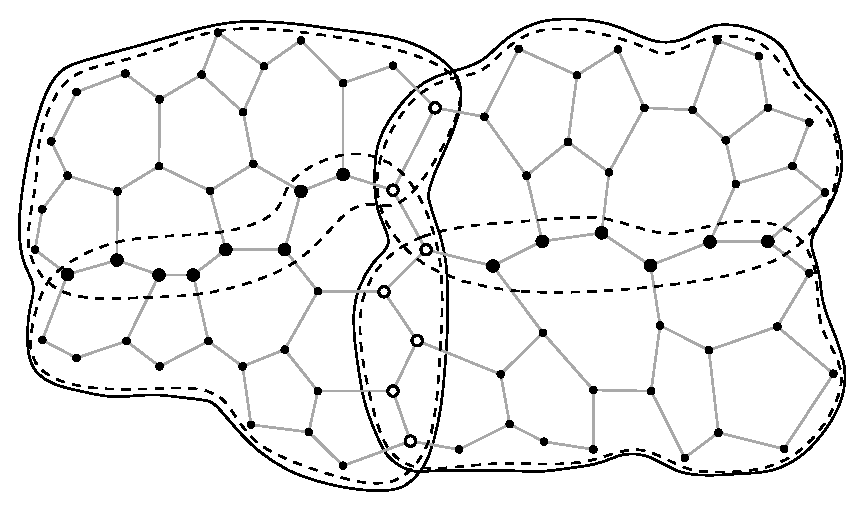
\includegraphics[width=0.6\textwidth]{Fig1}
  \caption[Recursively-partitioned graph]{A graph $G$ partitioned into two 
	regions (delineated by solid lines), which are further partitioned into two 
	subregions each (delineated by dashed lines).
    Region boundary vertices are shown as large hollow disks while subregion 
	boundary vertices interior to their regions are shown as large solid disks.
    Vertices interior to their subregions are shown as small solid disks}
  \label{fig:partitioned_graph}
\end{figure}
% ------------------------------------------------------------------------------

In our data structure, all subregions are stored explicitly while
regions are represented implicitly as unions of their subregions.
In addition, we store the \emph{$\alpha$-neighbourhoods} of all (region
and subregion) boundary vertices.
These neighbourhoods are defined
as follows~\cite{DBLP:conf/soda/AgarwalAMVV98}.
For a vertex $x$, consider a breadth-first search in $G$ starting at $x$.
Then the $\alpha$-neighbourhood $\nb[\alpha]{x}$ of $x$ is the subgraph of $G$
induced by the first $\alpha$ vertices visited by the search.
For a region boundary vertex, we store its entire $\alpha$-neighbourhood.
For a subregion boundary vertex interior to a region $\reg[i]$, we store
only those vertices of its $\alpha$-neighbourhood that belong to
$\reg[i]$.
A vertex $y \in \nb[\alpha]{x}$ is an \emph{interior vertex} of
$N_\alpha(x)$ if all its neighbours belong to $\nb[\alpha]{x}$;
otherwise $y$ is \emph{terminal}
(see Fig.~\ref{fig:alpha_neighbourhoods} for an illustration of the
definitions pertaining to $\alpha$-neighbourhoods).

% ------------------------------------------------------------------------------
\begin{figure}[t]
  \centering
  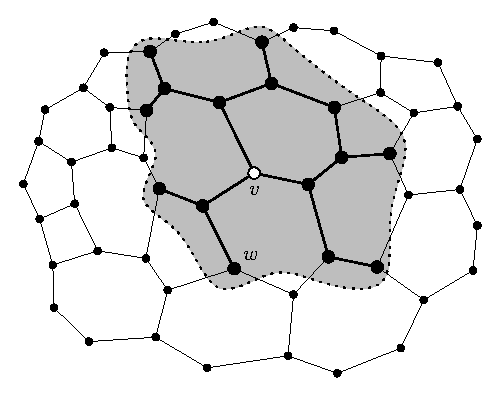
\includegraphics{Fig2}
  \caption[$\alpha$-neighbourhood of a boundary vertex]{The 
	$\alpha$-neighbourhood $\nb[\alpha]{v}$ of a vertex $v$,
    for $\alpha = 16$.
    Vertex $v$ is interior to $\nb[\alpha]{v}$ while vertex $w$ is terminal}
  \label{fig:alpha_neighbourhoods}
\end{figure}
% ------------------------------------------------------------------------------

We refer to subregions and $\alpha$-neighbourhoods---that is, to the
subgraphs of $G$ we store explicitly---as \emph{components} of $G$.
We store each component succinctly so as to allow for the efficient
traversal of edges in the component.
The traversal of a path in $G$ must be able to visit different components.
In order to facilitate this, we assign a unique \emph{graph label} to each vertex of $G$
and provide mechanisms to (1) identify a component containing a vertex $x$ and
locate $x$ in that component, given its graph label, and (2) determine
the graph label of any vertex in a given component.

The rest of this section is organized as follows.
In Section~\ref{sec:graph_labelling}, we define a number of labels
assigned to the vertices of $G$, including the graph labels just
mentioned, and provide $\ohOf{N}$-bit data structures that allow us to
convert any such label into any other label using $\OhOf{1}$ I/Os.
In Section~\ref{sec:datastructs}, we discuss the succinct
representations we use to store subregions and
$\alpha$-neighbourhoods.
In Section~\ref{sec:navigation},
we discuss how to traverse paths I/O efficiently using this
representation.
In Section \ref{sec:alt_block_scheme}, we describe an 
alternative scheme
for blocking bounded degree planar graphs that can improve I/O efficiency in 
some instances.

% ------------------------------------------------------------------------------
\subsection{Graph Labeling}
% ------------------------------------------------------------------------------

\label{sec:graph_labelling}

In this section, we describe the labeling scheme that underlies our
data structure.
Our scheme is based on the one used in
Bose~\etal~\cite{DBLP:journals/talg/BoseCHMM12}.
It assigns three labels to each vertex.
As already mentioned, the \emph{graph label} $\glbl{x}$ identifies each vertex
$x \in G$ uniquely.
The \emph{region label} $\reglbl[i]{x}$ of a vertex $x$ in a region $\reg[i]$
identifies $x$ uniquely among the vertices in $\reg[i]$, and the
\emph{subregion label} $\subreglbl[i,j]{x}$ of a vertex $x$ in a subregion
$\subreg[i,j]$ identifies $x$ uniquely
among the vertices in $\subreg[i,j]$.
(Note that a region boundary vertex appears in more than one region and,
thus, receives one region label per region that contains it.
Similarly, every region or subregion boundary vertex receives multiple
subregion labels.)

A standard data structure would identify vertices by their graph labels and
store these labels for every vertex.
Since there are $N$ vertices, every graph label must use at least
$\lg N$ bits, and such a representation uses at least $N \lg N$ bits of space.
In our structure, we store graph labels for only a small subset of the vertices, 
region labels for yet another subset of the vertices, and subregion labels for 
a third subset. 
Many vertices in the graph have no label explicitly stored.
Since regions and subregions are small, and region and subregion labels have to
be unique only within a region or subregion, they can be stored using
less than $\lg N$ bits each.
Next we define these labels.

In the data structure described in the next section, the vertices of
each subregion $\subreg[i,j]$ are stored in a particular order $\perm[i,j]$.
We use the position of a vertex $x$ in $\perm[i,j]$ as its
subregion label $\subreglbl[i,j]{x}$ for subregion~$\subreg[i,j]$.

For a region $\reg[i]$ and a vertex $x \in \reg[i]$, we say an occurrence of
$x$ in a subregion $\subreg[i,j]$ \emph{defines} $x$ if there is no
subregion $\subreg[i,h]$ with $h < j$ that contains~$x$; otherwise the
occurrence is a \emph{duplicate}.
If the occurrence of $x$ in a subregion $\subreg[i,j]$ defines $x$, we also call
$\reg[i,j]$ the \emph{defining subregion} of $x$.
Clearly, all occurrences of subregion interior vertices are
defining.
We order \footnote{This ordering, as with the ordering used for assigning 
graph labels, is employed strictly for labeling purposes. It does not imply
any arrangement of vertices within the structures used to represent the graph.}
the vertices of $\reg[i]$ so that all subregion boundary vertices
precede all subregion-interior vertices, and the vertices in each of these two
groups are sorted primarily by their defining subregions and secondarily by
their subregion labels within these subregions.
The region labels of the vertices in $\reg[i]$ are now obtained by numbering the
vertices in this order.


Graph labels are defined analogously to region labels.
Again, we say an occurrence of a vertex $x$ in a region $\reg[i]$ defines
$x$ if $x \not\in \reg[h]$, for all $h < i$.
We then order the vertices of $G$ so that the region boundary vertices precede
the region-interior vertices, and the vertices in each of these two groups are
sorted primarily by their defining regions and secondarily by their region
labels inside their defining regions.
The graph labels of the vertices in $G$ are
then obtained by numbering the vertices in order.

Observe that this labeling scheme ensures that all vertices interior
to a region $\reg[i]$ receive consecutive graph labels, and all vertices
interior to a subregion $\subreg[i,j]$ receive consecutive graph and
region labels.
Our data structure for representing the graph $G$ will make use of
the following result, which extends a result from \cite{DBLP:journals/talg/BoseCHMM12}.
In particular, parts~\ref{item:subregion-to-region}
and~\ref{item:region-to-graph} were proved in \cite{DBLP:journals/talg/BoseCHMM12} for a slightly
different vertex labeling than we use here while
parts~\ref{item:graph-to-region} and~\ref{item:region-to-subregion} are new.
For completeness, we prove all parts of the lemma here.

% ------------------------------------------------------------------------------
\begin{lemma}
  \label{lem:label_ops}
  There is a data structure of $\ohOf{N}$ bits that allows the following
  conversion between vertex labels of $G$ to be performed using
  $\OhOf{1}$ I/Os.
  \begin{enumerate}[label={(\alph{*})},noitemsep]
  \item Given the graph label $\glbl{x}$ of a vertex $x$, compute the defining
    region $\reg[i]$ of $x$ and the region label $\reglbl[i]{x}$ of $x$ in
    $\reg[i]$.\label{item:graph-to-region}
  \item Given the region label $\reglbl[i]{x}$ of a vertex $x$ in a region
    $\reg[i]$, compute the defining subregion $\subreg[i,j]$ of $x$ and the
    subregion label $\subreglbl[i,j]{x}$ of $x$ in
    $\subreg[i,j]$.\label{item:region-to-subregion}
  \item Given the subregion label of a vertex $x$ in a subregion
    $\subreg[i,j]$ of $\reg[i]$, compute the region label $\reglbl[i]{x}$
    of $x$ in $\reg[i]$.\label{item:subregion-to-region}
  \item Given the region label of a vertex $x$ in a region $\reg[i]$,
    compute the graph label $\glbl{x}$ of $x$.\label{item:region-to-graph}
  \end{enumerate}
\end{lemma}
% ------------------------------------------------------------------------------

\begin{proof}
  We construct separate $\ohOf{N}$-bit data structures in order to accomplish parts
  \ref{item:region-to-subregion} and~\ref{item:subregion-to-region}, and to
  accomplish parts \ref{item:graph-to-region} and~\ref{item:region-to-graph}.
  Since these data structures are very similar, we discuss those for
  parts \ref{item:region-to-subregion} and~\ref{item:subregion-to-region} in detail,
  and only provide a space analysis for the second structure.
  We use $\numv[i]$ to denote the number of vertices in region $\reg[i]$,
  $\numv[i,j]$ to denote the number of vertices in subregion $\subreg[i,j]$,
  $\dnumv[i] := \sum_{j=1}^{q_i} \numv[i,j]$ to denote the total number of
  vertices in all subregions of~$\reg[i]$, where $q_i$ is the number of
  subregions of region $\reg[i]$, and $\dnumv := \sum_{i=1}^t \dnumv[i]$ to
  denote the total number of vertices in all subregions.

  Our data structure for converting between region and subregion labels consists
  of a number of vectors.
  We introduce them as required for the operations we discuss.
  Most of these vectors are bit vectors representing a vector $\vvec$
  of the vertices in all subregions of $G$.
  We define this vector first.
  $\vvec$ is the concatenation of $t$ subvectors $\vvec[1], \vvec[2],
  \dots, \vvec[t]$ storing the vertices in the regions of $G$.
  Each such vector $\vvec[i]$ is itself the concatenation of
  subvectors $\vvec[i,1], \vvec[i,2], \dots, \vvec[i,q_i]$ representing
  the subregions of $\reg[i]$.
  Each such vector $\vvec[i,j]$ stores the vertices in $\subreg[i,j]$
  sorted by their subregion labels.
  Note that our data structure does not store $\vvec$.
  We only introduce it here as a reference for discussing the vectors our
  data structure does store.
  Throughout this proof, when we define a bit vector, we store it using
  the second part of Lemma~\ref{lem:rank_select} to support constant-I/O
  accesses to its elements, as well as constant-I/O $\rankopsym$ and $\selopsym$
  operations.

\begin{table*}[ht]
	\centering
		\begin{tabular}{ l | l}
			Operator & Description \\ \hline
			$\rankop[x]{S, i}$ & Returns the number of $x$'s in bit-vector $S$ up to
				position $S[i]$, where $x \in \{0,1\}$.\\
			$\selop[x]{S, r}$ & Returns the $r$\textsuperscript{th} $x$ in bit-vector $S$
				where $x \in \{0,1\}$.\\
			$\regpos{i}$ & Returns the first element of region $\reg[i]$ in $\vvec$. \\
			$\subregpos{i,j}$ & Returns the first element of sub-region $\subreg[i,j]$
				in $\vvec$. \\
			$\possubreg{i,p}$ & Returns the sub-region index $j$ from $\vvec$ where
				$p \in \reg[i]$. \\
			$\bdcount{i}$ & Calculates in $\vvec$ the number of sub-region boundary vertices
				in $\reg[i]$. \\ \hline
		\end{tabular}
	\caption{Summary of bit-vector operations used in this section }
	\label{tab:succ_operators}
\end{table*}

  % ------------------------------------------------------------------
  \paragraph{Locating subvectors.}
  % ------------------------------------------------------------------

  The first two vectors that our data structure stores are bit vectors
  $\fstofreg$ and $\fstofsubreg$ that
  allow us to identify, for a region $\reg[i]$, the index of the first
  element of $\vvec[i]$ in $\vvec$ and, for a subregion $\subreg[i,j]$,
  the index of the first element of $\vvec[i,j]$ in $\vvec$.
  Both vectors have length $\dnumv = \size{\vvec}$.
  The $k$th bit in $\fstofreg$ is $1$ if and only if $\vvec[][k]$ is the
  first element of $\vvec[i]$, for some region $\reg[i]$,
  and the $k$th bit of $\fstofsubreg$ is $1$
  if and only if $\vvec[][k]$ is the first element of $\vvec[i,j]$, for some
  subregion $\subreg[i,j]$.
  Using these two bit vectors, we can implement the following three operations
  using $\OhOf{1}$ I/Os.
  \begin{itemize}
  \item $\regpos{i}$ returns the index of the first element of $\vvec[i]$
    in $\vvec$ and is implemented as $\regpos{i} := \selop[1]{\fstofreg,i}$.
  \item $\subregpos{i,j}$ returns the index of the first element of $\vvec[i,j]$
    in $\vvec$ and is implemented as\\
    $\subregpos{i,j} := \selop[1]{\fstofsubreg,\rankop[1]{\fstofsubreg,\regpos{i}-1}+j}$.
  \item $\possubreg{i,p}$ returns the index $j$ of the subregion $\subreg[i,j]$
    of $\reg[i]$ such that $\vvec[][p]$ is an element of  $\vvec[i,j]$,
    provided $\vvec[][p]$ is an element of $\vvec[i]$.
    This operation can be implemented as
    $\possubreg{i,p} := \rankop[1]{\fstofsubreg,p} - \rankop[1]{\fstofsubreg,
      \regpos{i} - 1}$.
  \end{itemize}

  % ------------------------------------------------------------------
  \paragraph{Identifying subregion boundary vertices.}
  % ------------------------------------------------------------------

  The next two vectors we store, $\idxvec$ and $\bdvec$, help us decide whether
  a vertex is a subregion boundary vertex based only on its region or subregion
  label.
  This is useful because the conversion between region and subregion
  labels is done differently for subregion boundary and subregion-interior
  vertices.
  Vector $\idxvec$ is the concatenation of $t+1$ bit vectors
  $\idxvec[1], \idxvec[2], \dots, \idxvec[t+1]$.
  For $1 \le i \le t$, the subvector $\idxvec[i]$ has length equal to the
  number of subregion boundary vertices in $\reg[i]$.
  Its first bit is $1$, all other bits are $0$.
  The last subvector $\idxvec[t+1]$ stores a single $1$ bit.
  Vector $\bdvec$ is a bit vector of length $n'$.
  $\bdvec[][k] = 1$ if and only if $\vvec[][k]$ is a subregion boundary
  vertex.

  Now observe that a vertex $x$ with region label $\reglbl[i]{x}$ in region
  $\reg[i]$ is a subregion boundary vertex if and only if
  $\reglbl[i]{x}$ is no greater than the number of subregion boundary vertices
  in $\reg[i]$ because, in the ordering used to define
  the region labels of the vertices in $\reg[i]$, all subregion boundary
  vertices precede all subregion-interior vertices.
  In order to test this condition, we need to compute the number of subregion
  boundary vertices in $\reg[i]$, which we can do using $\OhOf{1}$ I/Os
  as $\bdcount{i} := \selop[1]{\idxvec,i+1} - \selop[1]{\idxvec,i}$.
 
  For a vertex $x$ with subregion label $\subreglbl[i,j]{x}$ in subregion
  $\subreg[i,j]$, observe that the subvector $\vvec[i,j]$ of $\vvec$
  stores the vertices of $\subreg[i,j]$ sorted by their subregion labels.
  Thus, $x$ appears at position $\subreglbl[i,j]{x}$ in $\vvec[i,j]$,
  which is position $k := \subregpos{i,j} + \subreglbl[i,j]{x} - 1$ in $\vvec$.
  The corresponding bit $\bdvec[][k]$ in $\bdvec$ is $1$ if and only if
  $x$ is a subregion boundary vertex.
  Thus, testing whether $x$ is a subregion boundary vertex requires calculating
  $\subregpos{i,j}$, which takes $\OhOf{1}$ I/Os followed by a single lookup
  in the bit vector $\bdvec$.

  % ------------------------------------------------------------------
  \paragraph{Subregion-interior vertices.}
  % ------------------------------------------------------------------

  For the set of subregion-interior vertices, the vectors we have already
  defined suffice to convert between region
  and subregion labels.

  Given a subregion-interior vertex $x$ in $\reg[i]$ and its region label
  $\reglbl[i]{x}$ in $\reg[i]$, observe that the subregion-interior vertices in
  $\reg[i]$ appear in $\vvec[i]$ sorted by their region labels, and
  that these are exactly the vertices in $\vvec[i]$ whose corresponding
  bits in $\bdvec$ are $0$.
  Thus, since subregion-interior vertices have greater region labels than
  subregion boundary vertices, we can find the position $k$ of the only
  occurrence of $x$ in $\vvec$ as
  $k := \selop[0]{\bdvec, \rankop[0]{\bdvec, \regpos{i} - 1} + \reglbl[i]{x} 
  - \bdcount{i}}$, which takes $\OhOf{1}$ I/Os to compute.
  Vertex $x$ belongs to the subregion $\subreg[i,j]$ such that
  $\vvec[][k]$ belongs to $\vvec[i,j]$.
  The index $j$ of this subregion is easily computed using $\OhOf{1}$ I/Os, as
  $j := \rankop[1]{\fstofsubreg,k} - \rankop[1]{\fstofsubreg,\regpos{i}-1}$.
  Since vertices in $\vvec[i,j]$ are sorted by their subregion labels in
  $\subreg[i,j]$, the subregion label of $x$ is the index of $\vvec[][k]$
  in $\vvec[i,j]$, which can be computed using $\OhOf{1}$ I/Os as
  $\subreglbl[i,j]{x} := k - \subregpos{i,j} + 1$.

  To compute the region label in $\reg[i]$ for a subregion-interior
  vertex $x$ in $\subreg[i,j]$, we perform this conversion in the reverse
  direction.
  Firstly, we find the position $k$ of $x$ in $\vvec$ as
  $k := \subregpos{i,j} + \subreglbl[i,j]{x} - 1$.
  Secondly, we compute the region label of $x$ in $\reg[i]$ as
  $\reglbl[i]{x} := \rankop[0]{\bdvec,k} - \rankop[0]{\bdvec,\regpos{i}-1} + \bdcount{i}$,
  which is correct by the argument from the previous paragraph.
  Thus, the conversion from subregion labels to region labels also takes
  $\OhOf{1}$ I/Os.

  % ------------------------------------------------------------------
  \paragraph{Subregion boundary vertices.}
  % ------------------------------------------------------------------

  For subregion boundary vertices in $\reg[i]$, the vectors we have defined so
  far cannot be used to convert between region and subregion labels, mainly
  because these vertices by definition appear more than once in $\vvec[i]$.
  On the other hand, there are only a few such vertices, which allows us to
  store their region and subregion labels explicitly.
  In particular, we store two vectors $\regvec$ and~$\subregvec$.
  Vector $\regvec$ is the concatenation of subvectors $\regvec[1], \regvec[2],
  \dots, \regvec[t]$, one per region $\reg[i]$ of $G$.
  The length of $\regvec[i]$ is the number of subregion boundary vertices
  in $\reg[i]$, and $\regvec[i][k]$ is the pair $(j,k')$ such that the
  subregion $\subreg[i,j]$ is the defining subregion of the vertex $x$
  with region label $k$, and $k'$ is $x$'s subregion label in $\subreg[i,j]$.
  We represent the index $j$ using $\lg \regsz$ bits, and the subregion
  label $k'$ using $\lg \subregsz$ bits.
  The length of vector $\subregvec$ equals the number of $1$s in vector
  $\bdvec$.
  $\subregvec[][k]$ is the region label of the vertex in $\vvec$ corresponding
  to the $k$th $1$ in $\bdvec$.
  We store each such region label in $\subregvec$ using $\lg \regsz$ bits.

  Now consider a subregion boundary vertex $x$ with region label
  $\reglbl[i]{x}$ in $\reg[i]$.
  The index of the entry in $\regvec$ storing the index of the defining
  subregion of $x$ and $x$'s subregion label in this subregion is 
  $k := \selop[1]{\idxvec,i} + \reglbl[i]{x} - 1$, which takes
  $\OhOf{1}$ I/Os to compute.
  Another I/O suffices to retrieve $\regvec[][k]$.

  Given a subregion boundary vertex $x$ with subregion label
  $\subreglbl[i,j]{x}$ in subregion $\subreg[i,j]$, the index of $x$ in
  $\vvec$ is $k := \subregpos{i,j} + \subreglbl[i,j]{x} - 1$.
  The corresponding bit $\bdvec[][k]$ in $\bdvec$ is $1$, and the
  region label of $x$ can be retrieved from
  $\subregvec[][\rankop[1]{\bdvec,k}]$, which takes $\OhOf{1}$ I/Os.

  % ------------------------------------------------------------------
  \paragraph{Space bound.}
  % ------------------------------------------------------------------

  The vectors $\fstofreg$ and $\fstofsubreg$ have length
  $n' = N + \OhOf{N / \sqrt{\subregsz}} = \OhOf{N}$ because their length
  equals that of $\vvec$; only subregion boundary vertices appear more
  than once in $\vvec$, and the total number of occurrences of subregion
  boundary vertices in $\vvec$ is $\OhOf{N / \sqrt{\subregsz}}$ by
  Lemma~\ref{lem:fred_graph_sep}.
  Every $1$-bit in such a vector corresponds to the start of a region
  or subregion.
  Thus, both vectors contain $\OhOf{N / \subregsz} = \ohOf{N}$ $1$s.
  By Lemma~\ref{lem:rank_select}(b), this implies that both vectors can
  be represented using $\ohOf{N}$ bits.

  The vector $\idxvec$ has length $\OhOf{N / \sqrt{\subregsz}} = \ohOf{N}$
  because every bit in $\idxvec$ corresponds to a unique subregion boundary
  vertex.
  Thus, by Lemma~\ref{lem:rank_select}(a), we can store $\idxvec$ using
  $\ohOf{N}$ bits.

  The vector $\bdvec$ has length $n' = \OhOf{N}$ and contains
  $\OhOf{N / \sqrt{\subregsz}}$ $1$s, one per occurrence of a subregion boundary
  vertex in a subregion.
  Hence, by Lemma~\ref{lem:rank_select}(b), we can store $\bdvec$ using
  $\ohOf{N}$ bits.

  Finally, the number of entries in vectors $\regvec$ and $\subregvec$ is
  bounded by the number of occurrences of subregion boundary vertices in
  subregions, which is $\OhOf{N / \sqrt{\subregsz}}$.
  Each entry in such a vector is represented using
  $\OhOf{\lg \regsz} = \OhOf{\lg\subregsz + \lg \lg N}$ bits.
  Thus, the total space used by these two vectors is
  $\OhOf{(N / \sqrt{\subregsz})(\lg \subregsz + \lg \lg N)}$,
  which is $\ohOf{N}$ because $\subregsz = B = \OmegaOf{\lg N}$.
  To summarize, the vectors we use to convert between region and subregion
  labels use $\ohOf{N}$ space and allow us to convert between these labels
  using $\OhOf{1}$ I/Os.
  This proves parts (b) and (c) of the lemma.

  % ------------------------------------------------------------------
  \paragraph{Conversion between region and graph labels.}
  % ------------------------------------------------------------------

  The data structure for conversion between region and graph labels is
  identical, with the following modifications.
  \begin{itemize}
  \item The vector $\vvec$ is the concatenation of $t$ subvectors
    $\vvec[1], \vvec[2], \dots, \vvec[t]$.
    Vector $\vvec[i]$ stores the vertices in region $\reg[i]$ sorted
    by their region labels.
  \item The $k$th bit in $\bdvec$ is one if and only if the vertex
    $\vvec[k]$ is a region boundary vertex.
  \item There is no need for vectors $\fstofsubreg$ and $\idxvec$.
    Instead, we store a single $(\lg N)$-bit integer counting the number
    of region boundary vertices of $G$.
  \item The entries in $\regvec$ are pairs of indices of defining
    regions and region labels in these regions, and the entries in
    $\subregvec$ are graph labels.
  \end{itemize}
  Using these modified vectors, the conversion between graph and region labels
  can be accomplished using straightforward modifications of the procedures
  described in this proof.

  Vectors $\fstofreg$ and $\bdvec$ have length
  $N + \OhOf{N / \sqrt{\regsz}} = \OhOf{N}$ and contain $\OhOf{N / \regsz}$ and
  $\OhOf{N / \sqrt{\regsz}}$ $1$s, respectively, which are both $\ohOf{N}$.
  Hence, by Lemma~\ref{lem:rank_select}(b), they can both be stored using
  $\ohOf{N}$ bits.
  The number of region boundary vertices is stored using $\lg N = \ohOf{N}$
  bits.
  Each entry in vectors $\regvec$ and $\subregvec$ uses $\OhOf{\lg N}$ bits
  of space, and the number of these entries is $\OhOf{N / \sqrt{\regsz}}$.
  Hence, the total size of these vectors is $\OhOf{(N / \sqrt{\regsz}) \lg N}$,
  which is $\ohOf{N}$ because $\regsz \ge B \lg^2 N = \OmegaOf{\lg^3 N}$.
  This proves parts (a) and (d) of the lemma.
\end{proof}

% ------------------------------------------------------------------------------
\subsection{Data Structures}\label{sec:datastructs}
% ------------------------------------------------------------------------------

Our representation of $G$ consists of three parts: (1) succinct
representations of the subregions, packed into an array $\ds$, (2)
succinct representations of the $\alpha$-neighbourhoods of boundary
vertices, packed into two array $\regnbvec$ and $\subregnbvec$, and (3) two
vectors $\regminvec$ and $\subregminvec$ recording the minimum graph labels of
the interior vertices in each region or subregion.
Throughout this section, we use total orders $\reglt$ and $\subreglt$ of the
regions and subregions of~$G$, respectively.
For two regions $\reg[i]$ and $\reg[j]$, we define $\reg[i] \reglt \reg[j]$ if
$i < j$.
For two subregions $\subreg[i,j]$ and $\subreg[i',j']$, we define
$\subreg[i,j] \subreglt \subreg[i',j']$ if $i < i'$ or $i = i'$ and $j < j'$.

% ------------------------------------------------------------------------------
\paragraph{Minimum graph labels.}
% ------------------------------------------------------------------------------

The first part of our data structure consists of two arrays $\regminvec$ and
$\subregminvec$.
The $k$\textsuperscript{th} position of $\regminvec$ stores the minimum graph
label of the interior vertices in region $\reg[k]$.
The $k$\textsuperscript{th} position in $\subregminvec$ stores the minimum graph label of the
interior vertices in the subregion $\subreg[i,j]$ at position $k$ in the
sequence of subregions defined by $\subreglt$.

% ------------------------------------------------------------------------------
\paragraph{Succinct encoding of subregions.}
% ------------------------------------------------------------------------------

We represent each subregion $\subreg[i,j]$ using four data structures:
\begin{enumerate}
\item Its number of vertices $\numv[i,j]$ stored in $\lg N$
  bits.\footnote{$\lg \subregsz$ bits would suffice; however it simplifies the
    analysis to use $\lg N$ bits.}
\item The graph structure of $\subreg[i,j]$ encoded succintly as
	$\graphrep[i,j]$, using the encoding of 
	\cite{DBLP:journals/siamcomp/ChiangLL05}.
  This encoding involves a permutation $\perm[i,j]$ of
  the vertices in $\subreg[i,j]$.
\item A bit vector $\bdvec[i,j]$ of length $\size{\subreg[i,j]}$ with
  $\bdvec[i,j][i] = 1$ if and only if the corresponding vertex in $\perm[i,j]$
  is a  (region or subregion) boundary vertex.
\item An array $\keyvec[i,j]$ of length $\size{\subreg[i,j]}$ that stores the
  $\bitsPerKey$-bit key for each vertex.
  These labels are stored according to the permutation $\perm[i,j]$.
\end{enumerate}
The representation of $\subreg[i,j]$ is the concatenation of $\numv[i,j]$,
$\graphrep[i,j]$, $\bdvec[i,j]$, and $\keyvec[i,j]$.

Let $\succblksize$ be the maximum integer such that a subregion with $\succblksize$
vertices can be encoded in this manner
(The exact value of $\succblksize$, and its relation to $B$, is
provided in Equation~\ref{eqn:block_size} in the proof of Lemma~\ref{lem:main_space}).
We choose the parameters of our two-level partition as $\regsz := \succblksize \log^3
N$ and $\subregsz := \succblksize$.
This ensures that every subregion fits in a disk block.
However, a given subregion may be much smaller, and storing
each subregion in its own disk block may be wasteful.
Instead, we pack the representations of all subregions into an array $\ds$,
without gaps, using a construction proposed 
in~\cite{DBLP:journals/algorithmica/DillabaughHM12} as follows.
The subregion representations in $\ds$ are ordered according to $\subreglt$
and the array $\ds$ is stored in consecutive disk blocks; the first
$\lg N$ bits of each block are reserved for a \emph{block offset}
value.
Note that the representation of each region $\subreg[i,j]$ is
distributed over at most two consecutive blocks in $\ds$.
If $\subreg[i,j]$ is distributed over two blocks $B_1$ and $B_2$,
the block offset of the second block, $B_2$, records the number of bits
of $\subreg[i,j]$ stored in $B_2$.
Any other block stores a block offset of~$0$.
In other words, the block offset of each block stores the starting
position of the first region $\subreg[i,j]$ in this block that is not
stored partially in the previous block.
Since we use $\lg N$ bits per block to store the block offset, each subregion
of size $\succblksize$ must be stored in at most $B \wsize - \lg N$ bits.
This representation of $\ds$ is illustrated in Figure~\ref{fig:block-packing}.
 

% ------------------------------------------------------------------------------
\begin{figure}[t]
  \centering
  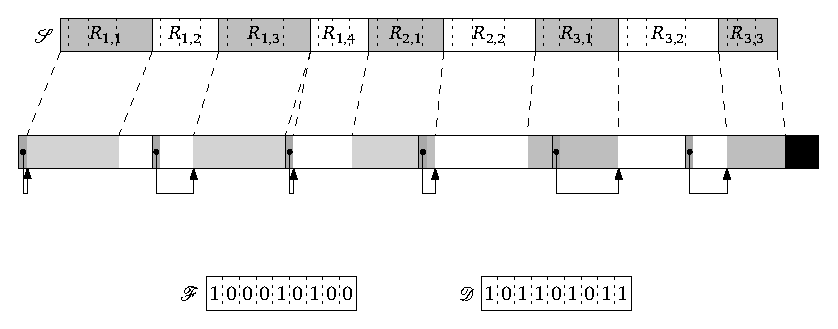
\includegraphics{Fig3}
  \caption[Packing graph blocks in memory]{Arrays $\ds$, $\fst$, and $\diff$ 
	and the packing of $\ds$ into blocks.
    The dark portion at the beginning of each block stores the block offset.
    The black portion of the last block is unused}
  \label{fig:block-packing}
\end{figure}
% ------------------------------------------------------------------------------

In order to facilitate the efficient lookup of subregions in $\ds$, we augment
it with two bit vectors $\fst$ and $\diff$, each represented to support
constant-time $\rankopsym$ and $\selopsym$ queries (see Lemma~\ref{lem:rank_select}).
If $Q$ is the total number of subregions in~$G$, each of the two vectors has
length $Q$.
Their entries are defined as follows:
\begin{enumerate}
\item $\fst[k] = 1$ if and only if the $k$th subregion $\subreg[i,j]$
  is the first subregion in $\reg[i]$; that is, if $j = 1$.
\item $\diff[k] = 1$ if and only if the $k$th subregion starts in
  a different block from the $(k-1)$st subregion, that is, if
  the first bits of these two regions belong to different blocks in
  $\ds$.
\end{enumerate}

% ------------------------------------------------------------------------------
\paragraph{\boldmath Succinct encoding of $\alpha$-neighbourhoods.}
% ------------------------------------------------------------------------------

The third piece of our data structure consists of succinct encodings
of the $\alpha$-neighbourhoods of (region and subregion) boundary
vertices, for $\alpha = (\succblksize)^{1/3}$.
Recall that the $\alpha$-neighbourhood of a subregion boundary vertex interior
to its region includes only vertices inside this region.
Each $\alpha$-neighbourhood $\nb[\alpha]{x}$ is represented using the
following structures:
\begin{enumerate}
\item A succinct encoding $\graphrep[x]$ of the graph structure of
  $\nb[\alpha]{x}$.
  This encoding involves a permutation $\perm[x]$ of the vertices in
  $\nb[\alpha]{x}$.
\item A bit vector $\term[x]$ of length $\size{\nb[\alpha]{x}}$ for which
  $\term[x][k] = 1$ if and only if the $k$th vertex in $\perm[x]$ is a terminal
  vertex of $\nb[\alpha]{x}$.
\item A $(\lg \alpha)$-bit integer $\pos[x]$ that records the position of
  $x$ in $\perm[x]$.
\item An array $\keyvec[x]$ of length $\size{\nb[\alpha]{x}}$ that stores the
  key associated with each vertex in $\nb[\alpha]{x}$.
  These keys are stored according to the permutation $\perm[x]$.
\item An array $\lblvec[x]$ of length $\size{\nb[\alpha]{x}}$ that stores
  labels of the vertices in $\nb[\alpha]{x}$.
  The specific labels stored in $\lblvec[x]$ depend on whether $x$ is a region
  boundary vertex or a subregion boundary vertex interior to a region.
  \begin{itemize}
  \item If $x$ is a region boundary vertex, $\lblvec[x][k]$ is the graph
    label of the $k$th vertex in $\perm[x]$.
    Each such graph label is stored using $\lg n$ bits.
  \item If $x$ is a subregion boundary vertex interior to a region
    $\reg[i]$, the label stored in $\lblvec[x][k]$ depends on the type of the
    $k$\textsuperscript{th} vertex $y$ in $\perm[x]$.
    If $y$ is an interior vertex of $\nb[\alpha]{x}$---that is,
    $\term[x][k] = 0$---then $\lblvec[x][k]$ is the difference between the graph
    label of $y$ and the minimum graph label of the interior vertices in
    $\reg[i]$,  which is stored in $\regminvec$.
    We call this the \emph{region offset} of $y$.
    If $y$ is a terminal vertex of $\nb[\alpha]{x}$---that is,
    $\term[x][k] = 1$---then $\lblvec[x][k]$ is the region label of $y$.
    We note that each of these two types of labels can be stored using
    $\lg \regsz$ bits.
    For region labels this is obvious, as each region has at most $\regsz$
    vertices.
    For region offsets, we observe that every interior vertex of
    $\nb[\alpha]{x}$ must also be interior to $\reg[i]$ because every
    boundary vertex of $\reg[i]$ has at least one neighbour outside of
    $\reg[i]$ and, hence, must be terminal for $\nb[\alpha]{x}$ (if it is
    contained in $\nb[\alpha]{x}$) because $\nb[\alpha]{x}$ contains only
    vertices in $\reg[i]$.
    The bound on the number of bits required to store region offsets now
    follows because $\reg[i]$ has at most $\regsz$ vertices, and all interior
    vertices of $\reg[i]$ receive consecutive graph labels.
  \end{itemize}
\end{enumerate}

Given that each $\alpha$-neighbourhood contains at most $\alpha$
vertices, there exist upper bounds, $\regub$ and $\subregub$, on the number of
bits required to encode the $\alpha$-neighbourhood of any region or
subregion boundary vertex, respectively.
We pad every $\alpha$-neighbourhood $\nb[\alpha]{x}$ to size $\regub$ or
$\subregub$ using extra bits, depending on whether $x$ is a region boundary
vertex.
We store the $\alpha$-neighbourhoods of all region boundary vertices in
an array $\regnbvec$, and the $\alpha$-neighbourhoods of all subregion boundary
vertices interior to their regions in an array $\subregnbvec$.
The $\alpha$-neighbourhoods in each array are ordered according to the graph
labels of their defining boundary vertices.

In order to be able to locate the $\alpha$-neighbourhoods of boundary vertices
in $\regnbvec$ and $\subregnbvec$, we store two bit vectors,
$\regbdvec$ and $\subregbdvec$, of length $N$ that support $\rankopsym$
and $\selopsym$ queries;
$\regbdvec[i] = 1$ if and only if the vertex with graph label $i$ is a region
boundary vertex; $\subregbdvec[i] = 1$ if and only if the vertex is a subregion
boundary vertex interior to its region.

% ------------------------------------------------------------------------------
\paragraph{Space analysis.}
% ------------------------------------------------------------------------------

Before discussing how to traverse a path in $G$ using this
representation, we prove a bound on its size.

% ------------------------------------------------------------------------------
\begin{lemma}
  \label{lem:main_space}
  The above representation of a bounded-degree planar graph $G$ with
  $N$ vertices, each with an associated $\bitsPerKey$-bit key, uses 
  $N \bitsPerKey + \OhOf{N} + \ohOf{N \bitsPerKey}$ bits.
\end{lemma}
% ------------------------------------------------------------------------------

\begin{proof}
  First we determine $\succblksize$.
  Let $c = \OhOf{1}$ be the number of bits per vertex used in the succinct
  representation $\graphrep[i,j]$ of the graph structure of each subregion
  $\subreg[i,j]$.
  Then the representation of each subregion uses at most 
  $N + (c + \bitsPerKey + 1)\succblksize$ bits.
  Since a block can hold $B \wsize$ bits, with the first $\lg N$ bits used
  for the block offset in $\ds$, we have
  \begin{equation}
    \label{eqn:block_size}
    \succblksize = \frac{B \wsize - 2 \lg N}{c + \bitsPerKey + 1},
  \end{equation}
  assuming for the sake of simplicity that $c + \bitsPerKey + 1$ divides 
  $B \wsize - 2 \lg N$.
  Now we analyze the space consumption of the different parts of our structure.

  \textit{Minimum graph labels.}  The arrays $\regminvec$ and $\subregminvec$
  together store $\OhOf{N / \succblksize}$ graph labels, each of size $\lg N$.
  By (\ref{eqn:block_size}) and because $\bitsPerKey = \OhOf{\lg N}$, 
  $\succblksize = \OmegaOf{B} = \OmegaOf{\lg N}$.
  Hence, these two arrays use $\OhOf{N}$ bits of space.

  \textit{Subregions.}  Storing every vertex once uses $N (c + \bitsPerKey + 1)
  = N \bitsPerKey + \OhOf{N}$ bits.
  However, boundary vertices are stored once per subregion in which they are 
  contained.
  By Lemma~\ref{lem:fred_graph_sep}, there are $\OhOf{N / \sqrt{\regsz}}$ region
  boundary vertices and $\OhOf{N / \sqrt{\subregsz}}$ subregion boundary
  vertices, counting each occurrence separately.
  Since $\regsz \ge \subregsz = \succblksize = \OmegaOf{\lg N}$, storing boundary
  vertices therefore requires
  \begin{equation*}
    \OhOfV{\frac{(c + \bitsPerKey + 1)N}{\sqrt{\succblksize}}} =
    \OhOfV{\frac{cN}{\sqrt{\succblksize}}} +
    \OhOfV{\frac{\bitsPerKey N}{\sqrt{\succblksize}}} = \ohOf{N} + \ohOf{N \bitsPerKey}
  \end{equation*}
  bits.
  In addition, we store a $(\lg N)$-bit size $\numv[i,j]$ for each
  subregion $\subreg[i,j]$.
  These numbers use $\OhOf{N \lg N / \succblksize} = \OhOf{N}$
  bits, as there are $\OhOf{N / \succblksize}$ subregions.
  In total, the size of array $\ds$ is $T := N \bitsPerKey + \OhOf{N} + \ohOf{N \bitsPerKey}$,
  excluding block offsets.
  There is one block offset of size $\lg N$ per block of $B \wsize =
  \OmegaOf{\lg^2 N}$ bits.
  Thus, the total space used by block offsets is $\OhOf{T / \lg N} = \ohOf{N \bitsPerKey}$.

  The final part of the representation of subregions is the vectors
  $\fst$ and $\diff$.
  Each vector stores one bit per subregion.
  Thus, their total size is $\OhOf{N / \succblksize} = \ohOf{N}$, and they can be stored
  in $\ohOf{N}$ space to support $\rankopsym$ and $\selopsym$ operations.
  In summary, we use $N \bitsPerKey + \OhOf{N} + \ohOf{N \bitsPerKey}$ bits to represent all
  subregions.

  \textit{$\alpha$-Neighbourhoods.}  We bound the sizes of the
  $\alpha$-neighbourhoods of region and subregion boundary vertices
  separately.
  By Lemma~\ref{lem:fred_graph_sep}, there are $\OhOf{N / \sqrt{\regsz}}$
  region boundary vertices.
  The representation of the $\alpha$-neighbourhood of each such vertex uses
  \begin{equation*}
    \lg \alpha + \alpha(c + 1 + \bitsPerKey + \lg N) = \OhOfV{(\succblksize)^{1/3} \lg N}
  \end{equation*}
  bits.
  Hence, the total size of the $\alpha$-neighbourhoods of all
  region boundary vertices stored in $\regnbvec$ is: 
  
  \begin{equation*}
    \OhOfV{\frac{N (\succblksize)^{1/3} \lg N}{\sqrt{\regsz}}} =
    \OhOfV{\frac{N (\succblksize)^{1/3} \lg N}{\sqrt{\succblksize \lg^3 N}}} =
    \ohOf{N}.
  \end{equation*}
  The $\alpha$-neighbourhood of every subregion boundary vertex is
  represented using
  \begin{equation*}
    \lg \alpha + \alpha(c + 1 + \bitsPerKey + \lg \regsz) = \OhOfV{(\succblksize)^{1/3} (\bitsPerKey + \lg
      \regsz)}
  \end{equation*}
  bits.
  Since there are $\OhOf{N / \sqrt{\subregsz}} = \OhOf{N / \sqrt{\succblksize}}$
  subregion boundary vertices, the total size of their
  $\alpha$-neighbourhoods stored in $\subregnbvec$ is therefore
  \begin{align*}
    \OhOfV{\frac{N (\succblksize)^{1/3} (\bitsPerKey + \lg \regsz)}{\sqrt{\succblksize}}} &=
    \OhOfV{\frac{N (\succblksize)^{1/3} \bitsPerKey}{\sqrt{\succblksize}}} +
    \OhOfV{\frac{N (\succblksize)^{1/3} \lg (\succblksize \lg^3 N)}{\sqrt{\succblksize}}}\\
    &= \ohOf{N \bitsPerKey}.
  \end{align*}
  The last equality follows because $\succblksize = \OmegaOf{\lg N}$.
  Together, arrays $\regnbvec$ and $\subregnbvec$ use $\ohOf{N \bitsPerKey}$ space.

  The bit vectors $\regbdvec$ and $\subregbdvec$ have length $N$ each and
  contain $\ohOf{N}$ 1 bits each.
  Thus, by Lemma \ref{lem:rank_select}(b), they
  can be stored in $\ohOf{N}$ bits.
  
  In summary, we use $\ohOf{N \bitsPerKey}$ bits to store all $\alpha$-neighbourhoods.
  By summing the sizes of the three parts of
  our data structure, we obtain the space bound claimed in the lemma.
\end{proof}

% ------------------------------------------------------------------------------
\subsection{Navigation}
% ------------------------------------------------------------------------------

\label{sec:navigation}

To traverse a path $\path$ in $G$, we use a strategy similar to that used
by Agarwal \etal~\cite{DBLP:conf/soda/AgarwalAMVV98},
alternately using subregions and $\alpha$-neighbourhoods in order to make
progress along $\path$.
We assume we are given a function, $\stepop$, that takes the graph label
and key of the current vertex, $x$, as an argument, and either reports that $x$
is the last vertex of $\path$ (in which case the traversal should stop), or outputs
the graph label and key of the successor of $x$ in $\path$.
To make this decision, $\stepop$ may
use state information computed during the traversal of $\path$ up to $x$
and needs access to the set of neighbours of $x$.
Therefore, the task of our traversal procedure is to ensure that, during each step
along $\path$, the neighbours of the current vertex are in memory.

Assuming, without loss of generality, that the start vertex of $\path$ is 
interior to a subregion~$\subreg[i,j]$.
This is easy to ensure initially by loading the
representation of $\subreg[i,j]$ into memory.
Then we follow the path $\path$ by repeated application of the $\stepop$ function
and by invoking the following paging procedure for each visited vertex before
applying $\stepop$ to it.
\begin{itemize}
\item If the current vertex $x$ is interior to the current component
  (subregion or $\alpha$-neighbourhood) in memory, we do not do
  anything, as all of $x$'s neighbours are in memory.
\item If the current component is a subregion $\subreg[i,j]$ and $x$ is a
  boundary vertex of $\subreg[i,j]$, or the current component is an
  $\alpha$-neighbourhood $\nb[\alpha]{y}$ and $x$ is a terminal vertex of
  $\nb[\alpha]{y}$, then $x$ has neighbours outside the current
  component.
  We load a component containing $x$ and all its neighbours into memory:
  \begin{itemize}
  \item If $x$ is a region or subregion boundary vertex, we load its
    $\alpha$-neighbourhood $\nb[\alpha]{x}$ into memory.
  \item If $x$ is interior to a subregion $\subreg[i',j']$, we load
    $\subreg[i',j']$ into memory.
  \end{itemize}
\end{itemize}

Our paging strategy ensures that, for every vertex $x \in \path$, we have
a succinct representation of a component of $G$ containing all
neighbours of $x$ in memory when $x$ is visited.
To show that this allows us to traverse any path of length $K$
using $\OhOf{K / \lg B}$ I/Os, we need to show that
(1) given the graph label of a vertex $x$, we can identify and load its
$\alpha$-neighbourhood, or the subregion $x$ is interior to, using $\OhOf{1}$
I/Os; (2) the graph labels of the vertices in the component currently
in memory and the graph structure of this component
can be determined without performing any I/Os; and (3) for every
$\lg B$ steps along path $\path$, we load only $\OhOf{1}$ components into memory.

Before proving these claims, we prove that we can efficiently convert between
graph, region, and subregion labels of a vertex $x$, and identify the region and
subregion to which $x$ is interior, or, if $x$ is a region or subregion boundary vertex,
the region or subregion which defines $x$.
The following lemma states this formally.
Its proof is the same as in~\cite{DBLP:journals/talg/BoseCHMM12}.
We include it here for completeness.

The results of the previous lemma lead to the following lemma.

% ------------------------------------------------------------------------------
\begin{lemma}
\label{lem:component_ios}
When the traversal algorithm encounters a terminal or boundary
vertex $v$, the next component containing $v$ in which the traversal
may be resumed can be loaded in $O(1)$ I/O operations.
\end{lemma}
% ------------------------------------------------------------------------------

\begin{proof}
Consider firstly the case of a boundary vertex, $v$, for a subregion.
The vertex may be a region or subregion boundary.
By Lemmas \ref{lem:label_ops}(c) and \ref{lem:label_ops}(d), the graph
label of $v$ can be determined in $O(1)$ I/O operations.
If $v$ is a region boundary vertex, this graph label serves as a direct 
index into the array of region boundary vertex $\alpha$-neighbourhoods 
(recall that all region boundary vertices are labeled with consecutive 
graphs labels).
Loading the $\alpha$-neighbourhood requires an additional I/O operation.

If $v$ is a subregion boundary vertex, the region and region
label can be determined by Lemma \ref{lem:label_ops}(a). 
By Lemma \ref{lem:label_ops}(d) we can determine the graph label. 
For the subregion boundary vertex, $v$, with graph label $\ell_G$, we can
determine the position of the $\alpha$-neighbourhood of $v$ in
$\N_S$ in $O(1)$ I/Os by $\rankop[1]{\bdvec, \ell_G}$.
In order to report the graph labels of vertices in the
  $\alpha$-neighbourhood, we must know the graph label of the first
  interior vertex of the region, which we can read from
  $\mathcal{L}_R$ with at most a single additional I/O operation.

  Further, consider the case of a terminal node in a
  $\alpha$-neighbourhood. If this is the $\alpha$-neighbourhood of a
  subregion boundary vertex, the region $R_i$, and region label are
  known, so by Lemma \ref{lem:label_ops}(d) we can determine the graph
  label and load the appropriate component with $O(1)$ I/O
  operations. 
  Likewise for $\alpha$-neighbourhoods of a region
  boundary vertex the graph label is obtained directly from the vertex
  key.

  Finally, we show that a subregion can be loaded in $O(1)$
  I/Os. 
  Assume that  we wish to load subregion $R_{i,j}$. 
  Let $r = \selop[1]{\mathcal{B}_R,i}$ mark the start of the region $i$. 
  We can then locate the block, $b$, in which the representation for
  subregion $j$ starts by $b=\rankop[1]{\mathcal{B}_S, r+j}$. 
  There may be other subregions stored entirely in $b$ prior to
  $R_{i,j}$. 
  We know that if $\mathcal{B}_S[r+j] = 0$ then $R_{i,j}$ is the
  first subregion stored in $b$ that has its representation start in
  $b$.  
  If this is not the case, the result of
  $\selop[1]{\rankop[1]{\mathcal{B}_S,r+j}}$ will indicate the position
  of $r$ among the subregions stored in $b$.  
  We can now read
  subregion $R_{i,j}$ as follows: 
  we load block $b$ into memory and
  read the block offset which indicates where the first subregion in
  $b$ starts. 
  If this is $R_{i,j}$, we read the subregion offset in order to
  determine its length, and read $R_{i,j}$ into memory, possibly
  reading into block $b+1$ if there is an overrun. 
  If $R_{i,j}$ is not
  the first subregion starting in block $b$, then we note how many
  subregions we must skip from the start of $b$, and by reading only
  the subregion offsets we can jump to the location in $b$ where
  $R_{i,j}$ starts. 
  The $\rankopsym$ and $\selopsym$ operations require
  $O(1)$ I/Os, and we read portions of at most two blocks $b$ and
  $b+1$ to read a subregion, therefore we can load a subregion with $O(1)$
  I/Os.
\end{proof}


% ------------------------------------------------------------------------------
\begin{lemma}
  \label{lem:report_int_labels}
  Given a subregion or $\alpha$-neighbourhood, the graph labels of
  all interior (subregions) and internal ($\alpha$-neighbourhoods)
  vertices can be reported without incurring any additional I/Os
  beyond what is required when the component is loaded to main memory.
\end{lemma}
% ------------------------------------------------------------------------------

\begin{proof}
  The encoding of a subregion induces an order on all vertices, both
  interior and boundary, of that subregion. Consider the interior
  vertex at position $j$ among all vertices in the subregion. 
  The position of this vertex among all interior vertices may be
  determined by the result of $\rankop[0]{\mathcal{B}, j}$. 
  Recall that graph labels assigned to all interior vertices in a subregion are
  consecutive; therefore, by adding one less this value to the
  graph label of the first vertex in the subregion, the graph label
  of interior vertex at position $j$ is obtained.

  For the $\alpha$-neighbourhood of a region boundary vertex, the graph
  labels from $\mathcal{L}_\alpha$ can be reported directly.  
  For the $\alpha$-neighbourhoods of subregion boundary vertices, we can
  determine from $\mathcal{L}_R$ the graph label of the first vertex
  in the parent region. 
  This potentially costs an I/O; however, we can pay
  for this when the component is loaded. 
  We can then report graph
  labels by adding the offset stored in $\mathcal{L}_{\alpha}$ to the
  value from $\mathcal{L}_R$.
\end{proof}

\begin{lemma}
  \label{lem:main_IO_bound}
  Using the data structures and navigation scheme described above, a
  path of length $K$ in graph $G$ can be traversed in $O \left(
    \frac{K}{ \lg{\succblksize} } \right)$ I/O operations.
\end{lemma}

\begin{proof}
  The $\alpha$-neighbourhood components are generated by performing a
  breadth-first traversal, from the boundary vertex $v$, which
  defines the neighbourhood. A total of $\succblksize^{1/3}$ vertices are added
  to each $\alpha$-neighbourhood component. Since the degree of $G$ is
  bounded by $d$, the length of a path from $v$ to the terminal
  vertices of the $\alpha$-neighbourhood is
  $\log_d{\succblksize^{1/3}}$. 
  However, for subregion boundary vertices, the
  $\alpha$-neighbourhoods only extend to the boundary vertices of the
  region, such that the path from $v$ to a terminal node may be less
  than $\log_d{\succblksize^{1/3}}$. 
  In the latter case the terminal vertex
  corresponds to a region boundary vertex.

  Without loss of generality, assume that traversal starts with an
  interior vertex of some subregion. Traversal will continue in the
  subregion until a boundary vertex is encountered, at which time the
  $\alpha$-neighbourhood of that vertex is loaded. In the worst case
  we travel one step before arriving at a boundary vertex of the
  subregion. If the boundary vertex is a region boundary, the
  $\alpha$-neighbourhood is loaded, and we are guaranteed to travel at
  least $\log_d{\succblksize^{1/3}}$ steps before another component must be
  visited.  If the boundary vertex is a subregion boundary, then the
  $\alpha$-neighbourhood is loaded, and there are again two possible
  situations. In the first case, we are able to traverse
  $\log_d{\succblksize^{1/3}}$ steps before another component must be visited. In
  this case, by visiting two components, we have progressed a minimum
  of $\log_d{\succblksize^{1/3}}$ steps. In the second case, a terminal vertex in
  the $\alpha$-neighbourhood is reached before $\log_d{\succblksize^{1/3}}$ steps
  are taken. This case will only arise if the terminal vertex
  encountered is a region boundary vertex. Therefore, we load the
  $\alpha$-neighbourhood of this region boundary vertex, and progress
  at least $\log_d{\succblksize^{1/3}}$ steps along the path before another I/O
  will be required.

  Since we traverse $\log_d{\succblksize^{1/3}}$ vertices with a constant number
  of I/Os, we visit $O \left( \frac{K}{ \lg{\succblksize} } \right)$ components
  to traverse a path of length $K$. By Lemma \ref{lem:component_ios},
  loading each component requires a constant number of I/O operations,
  and by Lemma \ref{lem:report_int_labels} we can report the graph
  labels of all vertices in each component without any additional
  I/Os. Thus, the path may be traversed in $O \left( \frac{K}{ \lg \succblksize }
  \right)$ I/O operations.
\end{proof}

\begin{theorem}
  \label{thm:planar_graph}
  Given a planar graph $G$ of bounded degree, where each vertex stores
  a key of $\bitsPerKey$ bits, there is a data structure that represents $G$ in
  $N\bitsPerKey +O(N) + o(N\bitsPerKey)$ bits and permits traversal of a path of length
  $K$ with $O \left( \frac{K}{ \lg{B} } \right)$ I/O operations.
\end{theorem}

\begin{proof}
  Proof follows directly from Lemmas \ref{lem:main_space} and
  \ref{lem:main_IO_bound}. We substitute $B$ for $\succblksize$, using
  Eq.~\ref{eqn:block_size} ($\succblksize = \Omega(B)$), as this is standard for
  reporting results in the I/O model.
\end{proof}

Due to the need to store keys with each vertex, it is impossible to
store the graph with fewer than $N\bitsPerKey$ bits.  The space savings in our
data structure are obtained by reducing the space required to store
the actual graph representation.
Agrawal~\etal~\cite{DBLP:conf/soda/AgarwalAMVV98} do not attempt to
analyze their space complexity in bits but, assuming they use
$\lg{N}$ bit pointers to represent the graph structure, their
structure requires $\OhOf{N \lg{N}}$ bits for any size $\bitsPerKey$. 
If $\bitsPerKey$ is
a small constant, our space complexity becomes $\OhOf{N} +
\ohOf{N}$.
In the worst case when $\bitsPerKey = \ThetaOf{\lg N}$, our 
space complexity is $\ThetaOf{N \lg N}$, which is asymptotically 
equivalent to that of Agarwal~\etal.
However, even in this case, our structure can save a significant amount
of space due to the fact that we store the actual graph structure with
$\OhOf{N}$ bits (the $N \bitsPerKey$ and $\ohOf{N\bitsPerKey}$ terms
in our space requirements are related directly to the space
required to store keys), compared to $\OhOf{N \lg N}$ bits in their
representation.

% ----------------------------------------------------------------------------
\subsection{An Alternate Blocking Scheme}\label{sec:alt_block_scheme}
% ----------------------------------------------------------------------------

In this section, we describe a blocking scheme based on that
of Baswana and Sen \cite{DBLP:journals/algorithmica/BaswanaS02}, which
allows us to improve the I/O efficiency of our data structure for some
planar graphs. 
As with the blocking strategy of
\cite{DBLP:conf/soda/AgarwalAMVV98} employed previously, this new
strategy recursively identifies a separator on the nodes of the graph
$G$, until $G$ is divided into regions of size $r$ which can fit on a
single block (in this context, region is used generically to refer to
the size of partitions in the graph as in Lemma
\ref{lem:fred_graph_sep}). However, rather than storing
$\alpha$-nieghbourhoods of size $\sqrt{r}$ for each boundary vertex,
larger $\alpha$-neighbourhoods are stored for a subset of the boundary
vertices. 
In order for this scheme to work, it is necessary that
boundary vertices be packed close together, in order that the selected
$\alpha$-nieghbourhoods cover a sufficiently large number of boundary
vertices. This closeness of boundary vertices is not guaranteed using
the technique of \cite{DBLP:conf/soda/AgarwalAMVV98}, but if the
alternate separator algorithm of Miller~\cite{miller_1986} is
incorporated, then region boundary vertices are sufficiently packed.

For an embedded graph $G=(V,E)$ with maximum face size $c$,
the separator result of Miller~\cite{miller_1986} is 
stated in Lemma~\ref{lem:miller_cycle_sep}.

\begin{lemma}[Miller~\cite{miller_1986}]\label{lem:miller_cycle_sep}
If $G$ is an embedded 2-connected planar graph consisting of $N$ vertices, then
there exists a balanced separator which is a single vertex, or a simple cycle
of size at most $2 \sqrt{2 \left\lfloor \frac{c}{2} \right\rfloor N}$,
where $c$ is the maximum face size.
\end{lemma}

Baswana and Sen~\cite{DBLP:journals/algorithmica/BaswanaS02}
construct a graph permitting {I/O}-efficient traversal by recursively
applying this separator.
If the separator is a single vertex $v$, then an $\alpha$-neighbourhood
is constructed for $v$ with $\alpha = B$. 
If the separator is a cycle, then the following rule is applied.
Let $r^{-}(k)$ be the minimum depth of a
breadth-first search tree of size $k$ built on any vertex $v \in
V$.
From this cycle every $\frac{r^{-}(s)}{2}$\textsuperscript{th}
vertex is selected, and an $\alpha$-neighbourhood is constructed 
by performing a breadth-first search from each of the selected 
vertices.
In this case, we let $\alpha=s$, where $s$ is
a number in the range $(\sqrt{B},B)$, a precise value that will be
defined shortly.
Vertices on the cycle which are not selected are associated with the
$\alpha$-neighbourhood constructed for the nearest selected vertex $v$.

Let $S(N)$ be the total space required to block 
the graph in this fashion.
This value includes both the space for blocks storing the
regions, and for those storing $\alpha$-neighbourhoods.
The value for $S(N)$ following recursive application of the 
separator defined in Lemma~\ref{lem:miller_cycle_sep} is
given by

\begin{equation}
  S(N) = c_1N + c_2\frac{\sqrt{c}N}{\sqrt{B}r^{-}(s)} s
\end{equation}

where $c_1$ and $c_2$ are constants independent of $s$.
In order to maximize $s$ while maintaining $S(N) = \OhOf{N}$,
select for $s$ the largest value $z \le B$ such that 
$z \le r^{-}(z)\sqrt{\frac{B}{c}}$.
This is achieved by choosing 
$s = \textbf{min}\left(r^{-}(s)\sqrt{\frac{B}{c}}, B \right)$.

This construction is summarized in the following lemma.

\begin{lemma}[\cite{DBLP:journals/algorithmica/BaswanaS02}]
  A planar graph $G$ of size $N$ with maximum face size $c$ 
  can be stored in
  $\BigOh{ \frac{N}{B} }$ blocks so that a path of length $K$ can
  be traversed using $\BigOh{ \frac{K}{ r^{-}(s) } }$ I/O operations
  where $s = \textbf{min}\left( r^{-}(s)\sqrt{\frac{B}{c}}, B \right)$.
\end{lemma}

Our succinct graph representation relies on a two-level partitioning of 
the graph.
Before determining a bound on the space for such a succinct representation,
it is useful to bound the total number of boundary vertices 
resulting from the recursive application of Miller's separator; this is 
done in Lemma~\ref{lem:cycle_sep_size}.

\begin{lemma}
  \label{lem:cycle_sep_size}
  For an embedded planar graph $G$ on $N$ nodes, with faces of
  bounded maximum size $c$, recursively partitioned into regions of
  size $r$ using the cycle separator algorithm of Miller
  \cite{miller_1986}, the separator $S$ has $\OhOf{N/\sqrt{r}}$
  vertices.
\end{lemma}

\begin{proof}
  Miller's simple cycle separator on a graph of $N$ nodes has size at
  most $2 \sqrt{ 2 \left\lfloor \frac{c}{2} \right\rfloor N}$, which
  is $\OhOf{\sqrt{N}}$ for constant $c$. At each step in the
  partitioning, $G$ is subdivided into a separator $|S| =
  \OhOf{\sqrt{N}}$, plus subsets $N_1$ and $N_2$, each containing at
  most $\frac{2}{3}N$ nodes, plus the separator. 
  Thus if $\frac{1}{3} \le \epsilon \le \frac{2}{3}$, 
  we can characterize the size of the
  resulting subsets by $|N_1| = \epsilon N + \OhOf{\sqrt{N}}$ and
  $|N_2| = (1-\epsilon)N + \OhOf{\sqrt{N}}$. Following the proof of
  Lemma 1 in \cite{Frederickson87}, the total separator size required to
  split $G$ into regions of size at most $N$ then becomes
  $\BigOh{\frac{N}{\sqrt{r}}}$.
\end{proof}

We now describe how this technique is applied in order to achieve a succinct graph
encoding. 
Let $S_\alpha$ be the set of separator vertices selected as boundary
vertices.
We distinguish between the region separator vertices, 
$S^{R}_\alpha$, and the sub-region separator vertices $S^{SR}_\alpha$.
Select every $\frac{r^{-}(s)}{2}$\textsuperscript{th} separator vertex 
for which to build an $\alpha$-neighbourhood. 
The $\alpha$-neighbourhoods are constructed for a subset of 
the boundary vertices.
Each boundary vertex, $v$, is assigned to a single $\alpha$-neighbourhood, namely
the $\alpha$-neighbourhood centred nearest $v$ (or possibly at
$v$, if $v$ was an element of $S^{R}_\alpha$ or $S^{SR}_\alpha$). 
The graph is then encoded using the encoding described in 
Section~\ref{sec:datastructs}, with two small additions.
We add two arrays; one for region boundaries, which we denote 
$\regptable$, and the second for subregion boundaries,
which we denote $\subregptable$.
The length of these arrays is equal to the number of region boundary 
vertices and the number of sub-region boundary vertices, respectively.
Each of $\regptable$ (and $\subregptable$) is an array of tuples, where
the first tuple element is an index into $\regnbvec$ ($\subregnbvec$), 
and the second tuple element records the position of the vertex within
its $\alpha$-neighbourhood. 
By adding these structures to our existing succinct encoding, we have the
 following lemma.

% ------------------------------------------------------------------------------
\begin{lemma}
\label{lem:ptable_ios}
When the traversal algorithm encounters a terminal or boundary
vertex $v$, the next component containing $v$ in which the traversal
may be resumed can be loaded in $O(1)$ I/O operations.
\end{lemma}
% ------------------------------------------------------------------------------

\begin{proof}
The proof of this lemma is the same as that in 
Lemma~\ref{lem:component_ios}, with the addition that we must
use $\regptable$ and $\subregptable$ to lookup the correct 
$\alpha$-neighbourhood and the position of boundary vertex $v$
within it.

We begin with the case of a region boundary vertex.
In Lemma~\ref{lem:component_ios} it was shown that for a region
boundary vertex, we can locate its graph label in $\OhOf{1}$ I/O
operations.
The graph label serves as a direct index into $\regnbvec$.
In the current case, we let the graph label of a region boundary
vertex serve as an index into $\regptable$.
The first element in the corresponding tuple is a pointer to the
$\regnbvec$, and the second element of the tuple indicates from where
to resume traversal.
Using $\regptable$ incurs at most a single additional I/O.
Thus, lookup for region boundary vertices takes $\OhOf{1}$ I/O 
operations.

For subregion boundary vertices, we apply the same indirection
to locate the proper $\alpha$-neighbourhood.
The result of the lookup $\rankop[1]{\bdvec, \ell_G}$, rather
than serving as a direct index into $\subregnbvec$, is used 
as an index into $\subregptable$.
The pointer stored in the first element of the returned
tuple can then be used to locate the correct $\alpha$-neighbourhood
in $\subregnbvec$. 
Again, this extra array lookup results in only a single 
additional I/O.
\end{proof}

\begin{lemma}\label{lem:cycle_sep_space}
  The representation described above of a bounded-degree planar graph $G$,
  with $n$ vertices, each with an associated $\bitsPerKey$-bit key, uses 
  $n\bitsPerKey + \OhOf{n} + \ohOf{n\bitsPerKey}$ bits.
\end{lemma}

\begin{proof}
By Lemma \ref{lem:cycle_sep_size}, our two-level partitioning results
in $\OhOf{N/\sqrt{\succblksize \lg^{3}N}}$ region boundary vertices, and
$\OhOf{N/\sqrt{\succblksize}}$ subregion boundary vertices. From the separators
we select every $\frac{r^{-}(s)}{2}$'th vertex to add to $S_{\alpha}$,
so that we have $|S^{R}_{\alpha}| = \BigOh{ \frac{N}{\sqrt{\succblksize \lg^{3}N}
    r^{-}(s)} }$ and $|S^{SR}_{\alpha}| = \BigOh{\frac{N}{\sqrt{\succblksize}
    r^{-}(s)} }$.

We now demonstrate that the succinct encoding of the data structures
required to represent this partitioning requires the same amount of
storage as our previous result. 
We now store fewer, but larger,
$\alpha$-neighbourhoods, and we must store the tables $\subregptable$ and
$\regptable$.
For $\subregptable$, the first pointer in the tuple points to a block 
associated with an $\alpha$-neighbourhood in
$S^{SR}_{\alpha}$, and therefore requires 
$\lg{ \left( \BigOh{\frac{N}{\sqrt{\succblksize} r^{-}(s)}} \right)}$ 
bits, while the
vertex pointer requires $\lg{\succblksize}$ bits. The total space requirement in
bits for $\subregptable$ is thus:

\begin{equation}
  \OhOf{N/\sqrt{\succblksize}} \cdot \left( \lg{\left( \OhOf{\frac{N}{\sqrt{\succblksize}
            r^{-}(s)}} \right)} + \lg{\succblksize}  \right) = \ohOf{N}
\end{equation}

For $\regptable$, the respective pointer sizes are
$\lg{\left( \BigOh{\frac{N}{\sqrt{\succblksize \lg^3{N} } r^{-}(s)}} \right)}$
and $\lg{\succblksize}$ bits and, similarly, the total space is $\ohOf{N}$
bits.

Finally, we must account for the space required for the
$\alpha$-neighbourhoods. Before doing so, we must determine the actual
size of the $\alpha$-neighbourhoods, which we will denote $s$. Let $s
= \textbf{min}\left(r^{-}(s)\frac{\succblksize^{1/3}}{\sqrt{c} }, \succblksize \right)$; 
we then have the following space complexities for region boundary
vertices (the term $k$ represents the constant from the $O()$
notation):

\begin{equation}
  \label{eqn:space_region_bound_scs}
  \frac{k\sqrt{c}N}{\sqrt{\succblksize \lg^3{N}} r^{-}(s)} \cdot
  r^{-}(s)\frac{\succblksize^{1/3}}{\sqrt{c} } \cdot ( \lg{N} + \bitsPerKey + c ) = o(N)
\end{equation}

% and subregion boundary vertices:

\begin{eqnarray}
\frac{k\sqrt{c}N}{\sqrt{\succblksize} r^{-}(s)} \cdot r^{-}(s)\frac{\succblksize^{1/3}}{\sqrt{c} } \cdot ( \lg{(\succblksize \lg^3{N})} + \bitsPerKey + c ) &=& \frac{kN}{\succblksize^{\frac{1}{6}}} (\lg{\succblksize} + 3 \lg{\lg{N}}) + \frac{kN}{\succblksize^{\frac{1}{6}}}(\bitsPerKey+c) \nonumber \\
&=& \OhOf{N} + \ohOf{N\bitsPerKey} \label{eqn:space_sub_reg_bound}
\end{eqnarray}

\end{proof}

These results match the space requirements obtained for region and
subregion $\alpha$-neighbourhoods using our original partitioning
scheme (see Eqs. \ref{eqn:space_region_bound_scs} and
\ref{eqn:space_sub_reg_bound}), and lead to the following theorem.

\begin{theorem}
  Given a planar graph $G$ of bounded degree and with face size
  bounded by $c$, where each vertex stores a key of $\bitsPerKey$ bits, there is
  a data structure representing $G$ in $N\bitsPerKey +O(N) + o(N\bitsPerKey)$ bits that
  permits traversal of a path of length $K$ with $O \left( \frac{K}{
      r^{-}(s) } \right)$ I/O operations, where $s =
  \textbf{min}\left(r^{-}(s)\frac{\succblksize^{1/3}}{\sqrt{c} }, \succblksize \right)$.
\end{theorem}

\begin{proof}
The succinct structure and navigation technique is the same as
described in Theorem~\ref{thm:planar_graph}.
The only change is the addition of $\subregptable$ and $\regptable$.
Lemma~\ref{lem:ptable_ios} demonstrates that the new structures do not alter the
bounds on I/Os, while Lemma~\ref{lem:cycle_sep_space} establishes that the 
space complexity is unchanged.
\end{proof}


% ------------------------------------------------------------------------------
\section{Triangulations Supporting Efficient Path Traversal}
\label{sec:tins}
% ------------------------------------------------------------------------------

In this section, we describe how our data structures may be used to 
represent triangulations in a manner that permits efficient path
traversal in the EM setting.
In Section \ref{ssec:triangulation_rep}, we describe this representation in the 
general, non-EM setting, giving a compact representation for triangulations 
based on succinct representations of planar graphs.
Later, in Section \ref{ssec:compact_tin_external}, we detail how our succinct
and I/O-efficient planar graph representation can be applied to this representation
to yield a compact representation for 
triangulations permitting I/O-efficient path traversal.

% -------------------------------------------------------------------------
\subsection{Representing Triangulations}
\label{ssec:triangulation_rep}
% -------------------------------------------------------------------------

Let $\pointset$ be a set of points in $\plane$, then the triangulation $\triang$
of $\pointset$ is the planar graph with $\pointset$ vertices and all faces 
(except the outer face) of size $3$.
The set of all edges adjacent to the outer face of the triangulation is the
convex hull of $\pointset$. 
Let $\triang = (\pointset,E,T)$ be the triangulation with vertices $\pointset$, 
edges $E$, and 
triangles (faces) $T$. 
The dual graph of $\triang$ is $\dual{\triang} = (T^*,E^*,\pointset^*)$, it has a node
 $t^* \in T^*$ for each triangle $t \in T$, a face $p^* \in \pointset^*$ for each 
vertex $p \in \pointset$, and an edge $e^* \in E^*$ connecting vertices $t^*_1$ and
 $t^*_2$, if and only if triangles $t_1$ and $t_2$ share an edge in $\triang$.

We further define the \emph{augmented dual graph} 
 $\augdual{\triang} = (\augdual{V} = (\pointset \cup \dual{T}), \augdual{E},
\augdual{F})$.
Figure \ref{fig:aug_tri} shows an example of a triangulation, its dual, 
and its augmented dual graph.
The vertex set of $\augdual{\triang}$ is formed by the union of the vertex set 
$P$ of $\triang$ and the nodes $\dual{T}$ of $\dual{\triang}$. 
We will distinguish between two types of vertices in $\augdual{\triang}$, 
dependening on from which set the vertex is drawn. 
The vertices taken from the dual graph, denoted $\augdual{T}$, 
are referred to as the \emph{triangle nodes}. 
The vertices drawn from the set of vertices in the primal, $\pointset$, 
are refereed   
to as the \emph{point vertices} and are denoted $\augdual{\pointset}$.

For the edges of $\augdual{\triang}$, we again distinguish two types
 of edges. 
The \emph{triangle edges} are exactly the edge set in the dual, $E^*$. 
A \emph{point edge} is added between a triangle node and a point vertex
 if the point vertex is one of the corresponding triangle's three vertices in 
 the primal. 
We denote this set $\augdual{E}$, and define it formally as
$\augdual{E} = \{\augdual{e} | \left( e^* \in E^* \right)
 \cup \left( \augdual{e}=( \augdual{p} \in \augdual{\pointset}, 
  \augdual{t} \in \augdual{T} ) \text{ and } p 
  \text{ adjacent to } t \text{ in } \triang \right) \} $,
where $p$ and $t$ are the vertex and triangle, respectively, corresponding to 
$\augdual{p} \in \augdual{\pointset}$ and $t^{\augdualsym} \in T^{\augdualsym}$. 
$\augdual{\triang}$ also contains a set of faces $F^{\augdualsym}$, but these faces 
do not figure in our discussion. 


For purposes of quantifying bit costs, we denote by $\bitsPerPoint = \OhOf{\lg{N}}$ 
the number of bits required to represent a point in our data structures. 
Many application for triangulations will not require that a key be stored 
with the triangles, so we assume there is no $q$ bit key associated 
with each triangle node. 
We show that the space used by keys in our graph structure is effectively 
the same as the space used by the point set in our triangulation, but that 
if we wish to maintain keys we can do so without significantly increasing 
the space used.

% -------------------------------------------------------------------------------- %
\begin{figure}
\centering
	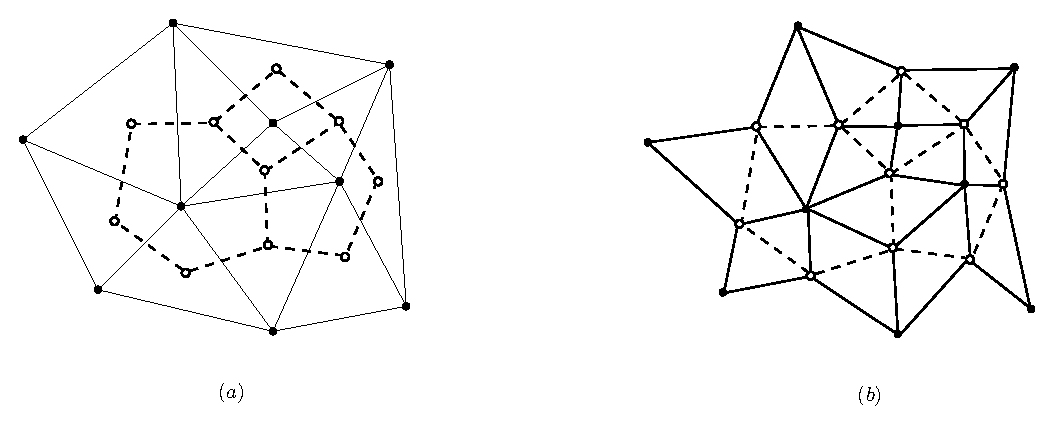
\includegraphics[width=0.8\textwidth]{Fig4}
\caption[Representation of a triangulation as a planar graph]{Representation 
	of a triangulation as a planar graph. 
  (a) The dual graph $\dual{\triang}$ of a triangulation, with vertices as hallow 
circles and edges as dashed lines. 
Edges in the triangulation $\triang$ are shown as solid lines. 
(b) The augmented graph $\augdual{\triang}$ is shown;
hallow points are triangle vertices, solid points are point 
vertices, black dashed lines are triangle edges, and solid lines are point 
edges }\label{fig:aug_tri}
\end{figure}
% ---------------------------------------------------------------------------------%

We begin with the following lemma which we state without proof. 

\begin{lemma}\label{lem:points_for_dual}
Given the dual graph, $\dual{\triang}$ of triangulation $\triang$ with 
$N$ triangles, the augmented dual graph $\augdual{\triang}$ has at most $2N+2$ 
vertices.
\end{lemma}

% Retain this for the THESIS.
%
\begin{proof}
The vertex set $\augdual{V}$ includes the nodes $\dual{T}$, for which 
$|\dual{T}| = N$, and the vertex set $\pointset$. 
We prove by induction that $|P| \le N+2$ and thus $|\augdual{V}| \le 2N + 2$. 
For the base case we have a terrain $\triang$ with a single triangle in which case 
$N = 1$ and $|P| = 3  = N + 2$. 
Now assume that $|P| \le N + 2$ holds for all terrains of $N$ triangles. 
Let $\dual{\triang}_N$ be the dual graph of a triangulation $\triang$ with $N$ 
triangles and $|P|$ vertices. 
The dual graph $\dual{\triang}_{N+1}$ is created by adding a single triangle 
to $\triang$. This new triangle, $t_1$, has three adjacent points, however, 
since $\dual{\triang}_{N+1}$ is connected, at least one dual edge is added 
connecting a vertex $t^*_2 \in \dual{\triang}_N$ with the new vertex 
$t^*_1 \in \dual{\triang}_{N+1}$. 
In $\triang$ this dual edge represents the fact that $t_1$ and $t_2$ are 
adjacent, and two of the vertices from $P$ adjacent to $t_2$ are already 
in $\augdual{V}$. Therefore, adding a new triangle adds at most one 
additional point to $\augdual{V}$ and $|\augdual{V}_{N+1}| \le (N+1) + 2$.
\end{proof}

We encode $\augdual{\triang}$ using a succinct planar graph data structure.
The various encodings all involve a permutation of the vertices of 
$\augdual{\triang}$.
Let $\ell(v)$, the \emph{augmented graph label} of $v \in \augdual{V}$, be 
the position of a vertex $v$ in this permutation. 
For every point vertex $p \in \augdual{P} \subset \augdual{V}$ in this set 
we store the point coordinates in an array $\mathcal{P}$ ordered by the 
augmented graph label, $\ell(p)$. 
We create a bit vector $\pi$ of length $|\augdual{V}|$, where 
$\pi[v] = 0$ if $v$ is a triangle vertex and $\pi[v] = 1$ if $v$ is a 
point vertex. 
To summarize this structure we have the following Lemma.

\begin{lemma}\label{lem:terrain_space}
The data structures described above can represent a triangulation, $\triang$, composed 
of $N$ triangles with $\bitsPerPoint = O(\lg{N})$ bit point coordinates, using 
$N\bitsPerPoint + O(N)$ bits, such that given the label of a triangle, the adjacent
 triangles and points can be reported in $O(1)$ time.
\end{lemma}

\begin{proof}
Since the augmented planar graph is simple, we can encode it with 
$2|\augdual{E}| + 2|\augdual{V}| + o(|\augdual{V}|)$ bits 
using the encoding of~\cite{DBLP:journals/siamcomp/ChiangLL05}. 
By Lemma \ref{lem:points_for_dual} if $|\dual{T}| = N$ then 
$|\augdual{V}| \le 2N+2$ which bounds the number of vertices. 
Each triangle node is connected by an edge to at most $3$ 
other triangles, so there are at most $\frac{3}{2} N$ triangle edges. 
Additionally, there are $3N$ point edges connecting the 
triangle vertices with point vertices, so in total there are no 
more than $\frac{9}{2}N$ edges. 
Thus the augmented graph can be encoded using at most $13N + o(N)$ bits. 

In~\cite{DBLP:journals/siamcomp/ChiangLL05} adjacency and degree queries
 can be performed in $O(1)$ time. 
We must still demonstrate that given a label we can identify the corresponding 
triangle vertex, and show that for a vertex we can distinguish between point 
vertex and triangle node neighbours. 
We assign to each triangle a unique graph label as follows. 
Consider the set of triangles in $\triang$, the graph label of each 
triangle corresponds to that of its dual vertex $t^* \in T^*$. 
In $\augdual{\triang}$ each of these vertices has an augmented graph label.  
The graph label of dual node $\dual{t} \in \dual{T}$, and therefore the 
corresponding triangle, is equal to the rank of the corresponding 
triangle vertex, $\augdual{t}$'s augmented graph label among all 
vertices from the set $\augdual{t}$. 

Given the graph label of a triangle node $\augdual{t} \in \augdual{T}$,
 the augmented graph label is calculated as $\ell(t^{\augdualsym}) = 
\selop[0]{\pi, \augdual{t}}$.
Conversely, given $\ell(\augdual{t})$ for a triangle vertex 
$\augdual{t} \in \augdual{T}$, we can report the graph label 
of $\augdual{t}$ by $\rankop[0]{\pi,\ell(\augdual{t})}$. 
To report the triangles adjacent to $\augdual{t}$, we check in 
the succinct encoding for $\augdual{\triang}$ to find all neighbours of 
$\augdual{t}$. 
Since $d \le 6$, this operation takes constant time. 
Let $\augdual{v} \in \augdual{V}$ be a neighbour of $\augdual{t}$ in 
$\augdual{\triang}$. 
The value of $\pi[\augdual{v}]$ indicates whether $\augdual{v}$ is a 
triangle node or point vertex. 
We can recover the coordinates of a point vertex $\augdual{v}$ by 
$\mathcal{P}[\rankop[1]{\pi,\augdual{v}}]$.

The array $\mathcal{P}$ stores at most $N+2$ points. 
If each point requires $\bitsPerPoint$ bits then $\mathcal{P}$ 
requires $N\bitsPerPoint$ bits. 
Finally, by Lemma \ref{lem:rank_select}(b) we can store the bit array 
$\pi$ such that $\rankopsym$ and $\selopsym$ can be performed in constant time 
with $N + o(N)$ bits.
\end{proof}

% -------------------------------------------------------------------------
\subsection{Compact External Memory Representation}
\label{ssec:compact_tin_external}
% -------------------------------------------------------------------------

In this section we extend our data structures for I/O efficient traversal in 
bounded degree planar graphs (Section \ref{sec:graph_rep}) to triangulations. 
We thereby obtain a triangulation that is compact, but which also 
permits efficient traversal. 
We represent $\triang$ by its dual graph $\dual{\triang}$. 
Since the dual graph of the the triangulation (and subsequently each component) is a 
bounded degree planar graph, it can be represented with the data structures 
described in Section \ref{sec:graph_rep}. 
Each component is a subgraph of $\dual{\triang}$, for which we generate the 
augmented subgraph, as described in Section~\ref{ssec:triangulation_rep}.

\begin{lemma}\label{lem:terrain_components}
The space requirement, in bits, to store a component ($\alpha$-neighbour-hood
 or sub-region) representing a triangulation is within a constant factor of the 
space required to store the triangulation's dual graph. 
\end{lemma}

\begin{proof}
We first consider the case of $\alpha$-neighbourhoods. 
To store a triangulation we require additional space to store: the points in $P$ 
adjacent to the component's triangles, the augmented 
graph, which includes more vertices and edges, and the bit-vector $\pi$. 
By Lemma~\ref{lem:points_for_dual} the points array is of size at most 
$(\alpha + 2)\bitsPerPoint$ bits. 
Since the $\alpha \bitsPerKey$-bit array of keys is no longer needed, storing the 
points incurs no additional space over that used to store the dual graph 
in our construction in Section \ref{sec:graph_rep}. 
However, if the keys are needed, we require 
$\alpha (\bitsPerPoint + \bitsPerKey)$ bits to 
store both the points and the key values.  
For the graph representation, again by Lemma \ref{lem:points_for_dual}, in 
the augmented graph we at most double the size of the vertex set and add 
no more than $3 \alpha$ edges. 
The graph encoding is a linear function of the number of edges and 
vertices. 
Therefore, the number of bits required for the graph encoding 
increases by a constant factor. 
Finally for $\pi$ we require fewer than two bits per vertex, so we can add 
this cost to the constant cost of representing the graph.

For sub-regions the analysis is more complex. 
A sub-region may be composed of multiple connected components, thus we cannot 
assume that there will be at most $\succblksize+2$ point vertices in the 
augmented subgraph.  
By Lemma \ref{lem:fred_graph_sep} there are no more than 
$\Theta(N/ \sqrt{\succblksize})$ boundary vertices in $\dual{\triang}$. 
Since each connected component in a sub-region must have at least one boundary vertex, 
this bounds the number of distinct connected components in all sub-regions. 
Each sub-region is composed of at most $\Theta(\sqrt{\succblksize})$ individual 
components, so in the worst case there are no more than 
$\sqrt{\succblksize}( \sqrt{\succblksize} + 2) < 2 \succblksize$ point vertices. 
Thus, the total number of vertices in the augmented graph is less than 
$3\succblksize$ which adds at most an additional $6\succblksize$ edges. 
As demonstrated with the $\alpha$-neighbourhoods, the additional storage, 
for all data structures used to represent a sub-region, 
increases by only a constant factor.
\end{proof}

One important feature of our representation is that each triangle stores 
very limited topological information. 
Consider the information available to some triangle 
$\augdual{t} \in \augdual{T}$ in the augmented dual graph. 
We can determine the - up to three - triangles adjacent to $\augdual{t}$, which 
correspond to the adjacent triangle vertices, as well as the three 
adjacent point vertices, but we have no information about how these are related.  
The only way to acquire this information is to actually visit each of 
$\augdual{t}$'s neighbours and thereby construct the topological 
information. 
Fortunately the need to visit the neighbours of a triangle in order to reconstruct 
its topological information will not increase the I/O costs of path traversal. 
If $\augdual{t}$ corresponds to an interior vertex (in a sub-region), or an 
internal vertex (in an $\alpha$-neighbourhood), then all of its neighbours are 
represented in the current component. 
If $\augdual{t}$ corresponds to a boundary (sub-region) or terminal 
($\alpha$-neighbourhood) vertex then the traversal algorithm already requires 
that a new sub-region, or $\alpha$-neighbourhood, be loaded. 
If we must load an $\alpha$-neighbourhood, then we are ensured all of 
$\augdual{t}$'s neighbours are in the new component. 
In the worst case $\augdual{t}$ is a terminal vertex in a 
$\alpha$-neighbourhood, and a boundary vertex in the newly loaded region. 
This forces us to load a second $\alpha$-neighbourhood, but observe that 
the same sequence of I/Os is necessary even if we were not required to 
reconstruct $\augdual{t}$'s local topology. 
Thus, at no point during a traversal is it necessary to load a component 
merely to construct the topology of a triangle in an adjacent, or overlapping,
component.

Due to Theorem~\ref{thm:planar_graph} and Lemma~\ref{lem:terrain_components} we
have the following theorem.

\begin{theorem}\label{thm:terrain_traversal}
Given triangulation $\triang$, where each point coordinate may be stored in 
$\bitsPerPoint$ bits, there is a data structure that represents $\triang$ in 
$N\bitsPerPoint + O(N) +o(N\bitsPerPoint)$ bits, that permits traversal of a path 
which crosses $K$ faces in $\triang$ with 
$O \left( \frac{K}{ \lg{B} } \right)$ I/O operations.
\end{theorem} 

For the case in which we wish to associate a $q$ bit key with each 
triangle we also have the following theorem.

\begin{theorem}\label{thm:terrain_keys_traversal}
Given triangulation $\triang$, where each point coordinate may be stored 
in $\bitsPerPoint$ bits, and where each triangle has associated with it a 
$\bitsPerKey$ bit key, there is a data structure that represents 
$\triang$ in 
$N(\bitsPerPoint + \bitsPerKey) + O(N) + o(N(\bitsPerPoint + \bitsPerKey))$ bits, that 
permits traversal of a path which crosses $K$ faces in $\triang$ 
with $O \left( \frac{K}{ \lg{B} } \right)$ I/O operations.
\end{theorem}

\begin{proof}
In our proof of Lemma \ref{lem:terrain_components} we demonstrated 
that the number of triangles (dual nodes with an associated $\bitsPerKey$ 
bit key) and points (of $\bitsPerPoint$ bits) are within a constant factor 
of each other in the worst case. 
Assuming this worst case does occur, we are effectively assuming each 
triangle is associated with a $\bitsPerKey$ bit key in our data structures. 
This yields the desired space bound.
\end{proof}




% ------------------------------------------------------------------------------
\section{Point Location for Triangulations}\label{sec:point_location}
% ------------------------------------------------------------------------------


A common operation in any partition of space is point location, or more
specifically in $\plane$, planar point location.
In Section \ref{sec:applications} we describe a number of queries
that require, as part of the query, identification of the triangle 
containing a point. 
For example, in order to perform a rectangular window query we start by
identifying the triangle containing one of the rectangle's four
corner points.
In this section we describe how to extend our data structure
for triangulations (see Section \ref{sec:tins}), in order to answer point 
location queries efficiently.

Our point location structure is based on that of 
Bose~\etal~\cite{DBLP:journals/talg/BoseCHMM12}.
One important difference between our technique and their's is that we use
a different data structure as the basis for performing point location.
Their construction relies on the point location structure of 
Kirkpatrick~\cite{DBLP:journals/siamcomp/Kirkpatrick83} for which there is no
known external memory version.  
We use the structure of Arge~\etal~\cite{DBLP:conf/alenex/ArgeDT03},
which uses linear space, and answers vertical ray shooting queries in 
$\OhOf{\log_B N}$ I/Os.

We want to design a point location structure which, given a query point $p_q$, 
will return the label of the subregion containing $p_q$. 
Since the subregion fits in internal memory, point location can be carried
out within the sub-region at no additional I/O cost.
We use a two-level search structure.  
The first level allows us to locate the region containing $p_q$, while the 
second allows us to locate the subregion containing $p_q$.
As the  structure is effectively the same at each level, we will only 
describe the structure for locating the region in detail.

Consider the set of region boundary vertices used to partition $\dual{\triang}$. 
These correspond to a subset of the triangles in $\triang$.
We select all the edges of this subset of the triangles of $\triang$,
and insert these into a search structure, which we denote $\N$.
With each edge in $\N$ we associate the label of the region
immediately below it.
If the triangle below an edge is shared by more than one region, as
will often be the case, we can arbitrarily select one. 
Our search structure $\N$ is built using the persistent B-tree structure of 
Arge~\etal~\cite{DBLP:conf/alenex/ArgeDT03} which answers vertical
ray shooting queries.
We repeat this process for each region, creating a search structure
$\N_i$ for each region $\reg[i]$.


In order to determine to which region the query point $p_q$ belongs to we perform a vertical 
ray shooting query from $p_q$ to report the first edge encountered in $\N$
above that point. 
Since we associate with each edge the region below it, the result of this query 
yields the region, $\reg[i]$ containing $p_q$.
We then search in $\N_i$ to locate the sub-region $j$ containing $p_q$.
Finally, we perform an exhaustive search on the triangles of $\subreg[i,j]$
to locate the triangle containing $p_q$.
It is possible, in the event that $p_q \notin \triang$, that the search yields
no result at the cost of searching $\N$, $\N_i$, plus the
the exhaustive search of $\subreg[i,j]$.
This is of course the same cost incurred by a successful search in the worst
case.

There is one important addition yet to make to the search structure $\N$.
Consider the situation depicted in Fig.~\ref{fig:pl_structure}(a), where
we wish to find the triangles containing points $p$ and $q$. 
The ray-shooting query from $p$ correctly returns an edge of the separator
vertically above it; however, the ray starting from $q$ never intersects a 
segment from the separator.

% ------------------------------------------------------------------------------
\begin{figure}
  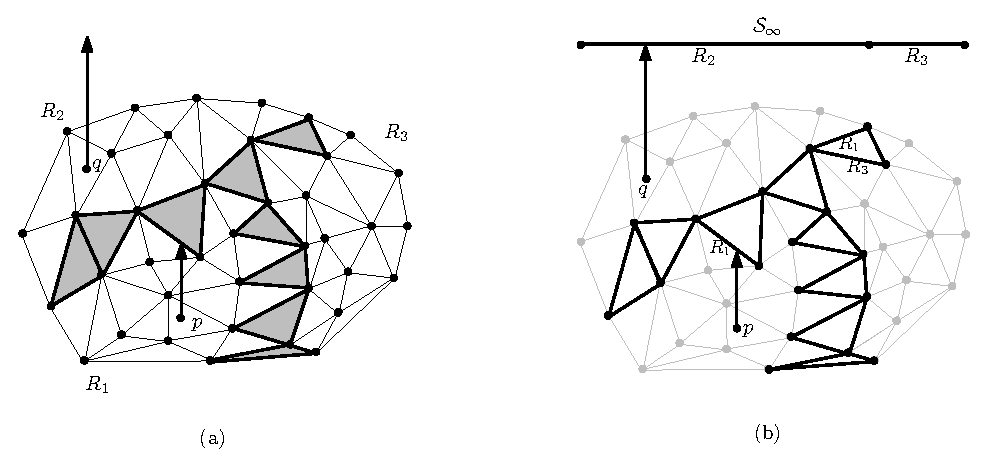
\includegraphics[width=\textwidth]{Fig5}
  \caption[Point location by vertical ray shooting]{In (a), a 
    partitioned triangulation is depicted along with two vertical
    ray shooting queries $p$ and $q$.
    Separator triangles between regions are shaded.
    Recall that the separator is calculated on the dual graph, thus
    the jagged appearance of the separator when drawn in the 
    triangulation.
    Inserting just the edges of boundary triangles into $\N$ is 
    sufficient to handle query $p$ but query $q$ fails.
    In (b), the complete search structure is shown.
    The segments added to $\N$ (heavy lines) 
    include all boundary triangle edges and the segments generated
    by partitioning $S_{\infty}$.
    Region labels for a small subset of $\N$ are indicated just below
    their respective segments
  }
  \label{fig:pl_structure}
\end{figure}
              
In order to ensure that the ray shooting query always reports a valid region, we 
extend our search structure $\N$ as follows.
Let $S_{\infty}$ be a line segment with endpoints at the min and max 
$x$ coordinates of $\triang$, and with $y$ coordinate $+\infty$.
We scan $\triang$ from left to right and split $S_{\infty}$ at any
point where the region immediately below the upper hull changes,
and record for each such segment the region immediately below.
If we insert all the newly-generated segments in $\N$, all vertical ray 
shooting queries within $\triang$ now return a valid result.

\begin{lemma}\label{lem:size_s_infty}
The number of segments added to $\N$ by partitioning $S_{\infty}$
is bounded by the size of the region separator for the subdivision
at the region level. Likewise, the number of segments added 
to all $\N_i$ is bounded by the size of the subregion separators.
\end{lemma}

\begin{proof}
We begin with proving this claim for $\N$.
By definition, $S_{\infty}$ is only split when the region immediately
below the upper hull of $\triang$ changes.
Any such change must occur at a vertex in $\triang$.
Let $v$ be this vertex and an let $t_i$ be a triangle in $\reg[i]$ 
immediately to its left, and $t_j$ a triangle in $\reg[j]$ immediately
to its right, where $t_i$ and $t_j$ are on the upper hull of
$\triang$ (see Fig.~\ref{fig:pl_s_infty}).
Assume for the sake of contradiction that none of the triangles
adjacent to $v$ is a boundary triangle. 
In our construction, no two edge adjacent triangles in $\triang$
can be in different regions unless at least on of them is
a boundary triangle.
Since $t_i$ and $t_j$ are in separate regions if we walk 
from $t_i$ to $t_j$ around $v$, we must arrive at two 
triangles which do not have the same region, since the
region label changes at some point along this walk.
This contradicts the claim that no triangle adjacent to $v$ is 
a boundary triangle.

The proof on the bound for the sizes of each $\N_i$ is 
analogous to that for $\N$.
There is one matter that must be addressed;
the separator algorithm of \cite{Frederickson87} does
not guarantee contiguous regions in $\triang$.
Within a region, this may introduce discontinuities 
that increase the complexity of $S_{\infty}$.
However, the number of such discontinuities is in no case
worse than the size of the region separator over
all $\N_i$. 

\end{proof}

% ----------------------------------------------------------------
\begin{figure}
  \centering
  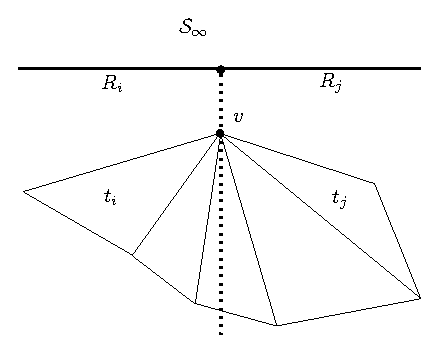
\includegraphics[scale=1.0]{Fig6}
  \caption[Bound on size of $\mathcal{S}_{\infty}$]{
  Illustration of proof that region boundary triangle must
  exists at a break in $S_{\infty}$
  }
  \label{fig:pl_s_infty}
\end{figure}
% ----------------------------------------------------------------


\begin{lemma}\label{lem:point_location_space}
By augmenting our terrain data structure with a structure using an additional 
$o(N\bitsPerPoint)$ bits, point location queries can be answered in 
$\OhOf{\log_{\succblksize}{N}}$ I/Os.
\end{lemma}

\begin{proof}
In the top level, region finding, data structure there are 
$\BigOh{ \frac{N}{\sqrt{\succblksize \lg^3 N}} }$ region boundary vertices. 
For each such vertex we insert at most six edges into our search structure;
this includes three edges for each triangle in the separator, plus any edges
added to $S_{\infty}$ by Lemma~\ref{lem:size_s_infty}.
Associated with each edge we must store $2\bitsPerPoint$ bits for the endpoints, 
plus a region label requiring $\lg{ \left( \frac{N}{\succblksize \lg^3 N} \right) }$ 
bits. 
Thus the total space, in bits, required by this structure will be:

\begin{eqnarray}
O\left( \frac{N}{\sqrt{\succblksize \lg^3{N}}} \right) \cdot \left( 2\bitsPerPoint + 
\lg{\left( \frac{N}{\succblksize \lg^3 N} \right)} \right) &=&  
O\left( \frac{N\bitsPerPoint}{\sqrt{\succblksize \lg^3 N}} \right) + 
\OhOf{\frac{N}{\sqrt{\succblksize \lg^3 N}}} \cdot 
\lg{ \left( \frac{N}{\succblksize \lg^3 N} \right) } \nonumber \\
	&=& \ohOf{N\bitsPerPoint} + \ohOf{N} \label{eqn:pl_region_space}
\end{eqnarray}

For the subregion search structures we will consider their space cumulatively.
We add $\OhOf{N/\sqrt{\succblksize}}$ edges, each requiring $2\bitsPerPoint$ bits
for the endpoints,
and $\lg{( \lg^3 N )}$ bit references to the $\lg^3{N}$ sub-regions within the region. 
Again, by Lemma~\ref{lem:size_s_infty}, the addition of edges in $S_{\infty}$ does not 
asymptotically increase the size of the $\N_i$.
The space required for this structure is then:

\begin{equation}\label{eqn:pl_subregion_space}
\BigOh{\frac{N}{\sqrt{\succblksize}}} \cdot ( 2\bitsPerPoint + \lg{(\lg^3{N})} ) = 
\BigOh{ \frac{N\bitsPerPoint}{\sqrt{\succblksize}}} + \BigOh{ \frac{N}{\sqrt{\succblksize}} \cdot \lg{\lg{(N)}}}
\end{equation}

The first term of this equation is clearly $\ohOf{ N \bitsPerPoint }$. 
Recall that $\succblksize = (B \lg N)/(c + \bitsPerPoint)$ and that $B = \OmegaOf{\lg{N}}$. 
Thus, for the second term of Eq.(\ref{eqn:pl_subregion_space}) we have:

\begin{eqnarray}
\BigOh{ \frac{N}{\sqrt{\succblksize}} \cdot 3 \lg{\lg{N}} } &=& 
\BigOh{ \frac{N}{\sqrt{\frac{B \lg N}{c+\bitsPerPoint}}} \cdot \lg{\lg{(N)}} } \nonumber\\
%&\le& \OhOf{ \frac{N\bitsPerPoint}{\sqrt{\lg^2{N}} } \cdot \lg{\lg{N}} } \nonumber\\
&=& \ohOf{N\bitsPerPoint}\label{eqn:pl_subregion_space_final}
\end{eqnarray} 

The total space we use is thus bounded by $\ohOf{ N\bitsPerPoint}$ bits. 
The I/O complexity stems from the fact that we perform two point location 
queries on data structures that answer the query in $\OhOf{\log_B N}$ I/Os.
\end{proof}

\begin{theorem}\label{thm:terrain_with_point_location}
Given a terrain $\triang$, where each point coordinate may be stored in $\bitsPerPoint$ 
bits, there is a data structure that represents $\triang$ in 
$N\bitsPerPoint + O(N) +o(N\bitsPerPoint)$ bits that permits traversal of a path crossing 
$K$ faces in $\triang$ with $O \left( \frac{K}{ \lg{B} } \right)$ I/Os, and 
supports point location queries with $\OhOf{\log_B{N}}$ I/Os.
\end{theorem} 

\begin{proof}
The terrain data structure requires $N\bitsPerPoint + O(N) +o(N\bitsPerPoint)$ bits by 
Theorem \ref{thm:terrain_traversal}. 
By Lemma \ref{lem:point_location_space}, adding point location requires only 
$\ohOf{N\bitsPerPoint}$ bits, thus the overall space bound is the same and queries 
can be answered in $\OhOf{\log_B{N}}$ I/Os.
\end{proof}



  % ------------------------------------------------------------------------------
  \section{Applications}
  \label{sec:applications}
  % ------------------------------------------------------------------------------

  In this section, we present a number of applications involving path traversal
  in triangulations.
  These applications employ the data structures described in Sections \ref{sec:tins}
  and \ref{sec:point_location}.
  The applications, in particular those described in 
  Section~\ref{ssec:ter_profile_tpath}, deal with triangulations used to model 
  terrains.
  A terrain model is a digital model of some surface.
  Most often the surface being modeled is some region of the earth, but any surface
  with relief can be modeled.
  Triangulations, commonly refered to as Triangular Irregular Networks, or TINs 
  in this context, are one means of modeling a digital terrain.
  In a TIN, the point set $\pointset$ is a set of points of known elevation. 
  Given a triangulation, $\triang$, built on $\pointset$, the elevation for any
  point, say $q$, on the surface can be readily estimated from the vertices
  of the triangle containing $q$.
  In addition to $x$ and $y$ coordinates, each point in $\pointset$ stores a $z$
  coordinate which records the elevation.
  Such models are sometimes refered to as 2.5 dimensional, since they cannot 
  properly represent a truly three-dimensional surface (for example there is no
  way for a planar triangulation to represent an overhanging cliff). 

  We begin by describing two simple and closely related queries, 
  reporting terrain profiles, and trickle paths, in 
  Section~\ref{ssec:ter_profile_tpath}.  
  In Section~\ref{sec:con_comp_queries}, we present a slightly more complex 
  application of our data structures, 
  reporting connected components of a triangulation (or terrain). 
  We start with the simpler case of reporting a component which is a convex
  subregion of the triangulation, and then describe methods for the more 
  general case where the connected component may represent a non-convex region.
  As all the queries we describe in this section require that a starting 
  triangle in the mesh be identified, we will assume that this triangle
  is given as part of the query.
  In practice, most of the queries we describe here can use a start triangle,
  identified by answering a
  single planar point location query using the technique outlined in 
  Section~\ref{sec:point_location}.

  \subsection{Terrain Profiles and Trickle Paths}\label{ssec:ter_profile_tpath}

  Terrain profiles are a common tool in GIS visualization. 
  The input is a line segment, or chain of line segments possibly forming a polygon, 
  and the output is a profile of the elevation along the line segment(s). 
  The trickle path, or path of steepest descent, from a point $p$ is the path on
  the terrain, represented by $\triang$, 
  that begins at $p$ and follows the direction of steepest descent until it reaches 
  a local minimum or the boundary of $\triang$ \cite{DBLP:conf/cccg/BergBDKOGRSY96}. 
  Both queries involve traversing a path over $\triang$, with the fundamental 
  difference being that in the terrain profile the path is given, whereas in 
  reporting the trickle path, the path is unknown beforehand and must be 
  determined based on local terrain characteristics.

  In analyzing these algorithms, we measure the complexity of a path by length 
  of the sequence of triangles visited, which we denote by $K$. 
  When a path intersects a vertex, we consider all triangles adjacent to that 
  vertex to have been visited. 
  Given this definition, we have the following result for terrain profile and 
  trickle path queries:

  \begin{lemma}\label{lem:tprofile_tpath}
  Let $\triang$ be a terrain stored using the representation described
  in Theorem~\ref{thm:terrain_traversal}, then:
  \begin{enumerate}[label={(\alph{*})}]
  \item{ Given a chain of line segments, $S$, the profile of the intersection 
  of $S$ with $\triang$ can be reported with $\BigOh{ \frac{K}{\lg{B}} }$ I/Os.}
  \item{ Given a point $p$ the trickle path from $p$ can be reported with 
  $\BigOh{ \frac{K}{\lg{B}} }$ I/Os.}
  \end{enumerate}
  \end{lemma}

  \begin{proof}
  Let $S$ be a chain of $i$ segments, denoted $s_0, s_1, \ldots s_i$. 
  In order to report an elevation profile, start at the endpoint of $s_0$, and 
  let $t \in \triang$ be the triangle which contains this endpoint. 
  We calculate the intersection of $s_0$ with the boundary of $t$ in order to determine 
  which triangle to visit next. 
  If at any point in reporting the query the next endpoint of the current segment 
  $s_j$ falls within the current triangle, we advance to the next segment 
  $s_{j+1}$. 
  This procedure is repeated until the closing endpoint of $s_i$ is reached.
  This query requires walking a path through $T$ that visits exactly $K$ triangles.

  For the trickle path, we are given triangle $t$ and some point interior to $t$. 
  The trickle path from $p$, and its intersection with the boundary of $t$, 
  can be calculated from the coordinates of the point vertices adjacent to $t$. 
  If the path crosses only the faces of triangles, we can simply report the 
  intersection of the path with those triangles.
  By Theorem \ref{thm:terrain_traversal}, it 
  requires $O(K/\lg{B})$ I/Os to report a path crossing $K$ triangles. 
  When an edge is followed, visiting both faces adjacent to that edge no more 
  than doubles the number of triangles visited. 
  The only possible problem occurs when the path intersects a point vertex. 
  Such cases require a walk around the point vertex to determine through which 
  triangle 
  (or edge) the path exits, or if the point vertex is a local minima. 
  In this case, the path must visit each triangle adjacent to the point vertex 
  through which it passes, thus all triangles visited during the cycle around a 
  point vertex are accounted for in the path length $K$.
  \end{proof}

  % -------------------------------------------------------------------------
  \subsection{Connected Component Queries}\label{sec:con_comp_queries}
  % -------------------------------------------------------------------------

  In this section, we describe how connected component queries can be reported 
  using our data structures. 
  We begin by defining \emph{connected component} and \emph{connected
  component query} in this setting.
  Let $\triang$ be a triangulation, and let $t$ be a triangle in $\triang$. 
  We denote by $\mathcal{P}(t)$ some property that is true for $t$.
  This property may be some value stored for each triangle, or some value that
  can be computed locally, such as slope or aspect if $\triang$ is a terrain.
  The connected component of $t$ with respect to $\mathcal{P}$ is the 
  subset $\concomp \subset \triang$, such that following conditions hold for
  all $t_c \in \concomp$:

  \begin{enumerate}
    \item $\mathcal{P}(t_c)$ is true, and
    \item there exists a path $t_1, t_2, \ldots t_n$ where $t = t_1$ and 
    $t_c = t_n$ such that $\mathcal{P}(t_i)$ is true for all $i$, and $t_i$ 
    and $t_{i+1}$ are adjacent.
  \end{enumerate}

  In order to simplify the discussion that follows, we adopt two conventions that we use
  throughout this section. 
  Firstly, while we assume that $\triang$ is represented by its augmented dual
  graph $\augdual{\triang}$, we will describe the various algorithms in terms
  of operations on the dual graph $\dual{\triang}$. 
  Furthermore, when we can do so without confusion, we use a single identifier
  to represent both a triangle and its corresponding node in the dual.
  For example, if we have triangle $t \in \triang$ corresponding to  
  $\dual{t} \in \dual{\triang}$, we may use $t$ in reference to both the
  triangle and the dual node.

  The second convention we will adopt relates to $\mathcal{P}$.
  If $\mathcal{P}(t)$ is true, then we call $t$ a \emph{red} node (triangle).  
  If $\mathcal{P}(t)$ is false, then we call $t$ a \emph{black} node (triangle).

  In Section~\ref{ssec:conv_con_comp} we address queries 
  where the component being reported is convex. 
  This constraint is not as limiting as it may seem.
  For example, rectangular window queries, a very common type of query, 
  may be viewed as a specialized case of reporting a convex 
  component.
  In Section~\ref{ssec:gen_con_comp}, we deal with the more challenging 
  problem of reporting
  connected components where the component may be non-convex.

  % -------------------------------------------------------------------------
  \subsubsection{Convex Connected Components}\label{ssec:conv_con_comp}
  % -------------------------------------------------------------------------

  Before describing the reporting of convex connected components, we show how 
  to solve a related problem. 
  Given the dual of a convex triangulation, $\dual{\triang}$, and a 
  vertex $\dual{s} \in \dual{\triang}$, 
  perform a depth-first traversal of $\dual{\triang}$, starting at $s$, without 
  using mark bits.
  Mark bits are commonly used in depth-first traversal to record which vertices 
  have already been visited. 
  However, their use is infeasible with our data structures, due to the 
  duplication of the vertices of $\dual{\triang}$.
  Mark bits would require that we find and mark all duplicates of 
  a vertex whenever it is visited.
  This entirely defeats the purpose of our data structure.

  In order to avoid the use of mark bits, we select from among the edges incident 
  to each node a single \emph{entry} edge for that node. 
  While performing a depth-first traversal, we extend the traversal 
  to a node only along its entry edge.
  This leaves us with the problem of determining how to select the entry edge
  for a node.  
  Gold and Maydell~\cite{gold_maydell_1978} and Gold and 
  Cormack~\cite{gold_cormack86} demonstrated how such an entry edge could 
  be selected to enable depth-first traversal on a triangulation.
  Their approach identified one of the three edges of a triangle as its 
  entry edge.
  Since there is a one-to-one correspondence between the edges in $\triang$ 
  and $\dual{\triang}$, we can apply such a rule to identifying entry
  edges for nodes in $\dual{\triang}$. 
  De~Berg~\etal~\cite{deberg_et_al_1997} showed that the same technique can 
  be applied to the more general case of planar subdivisions, and 
  gave an entry-edge selection rule for polygons that, naturally, also works 
  for triangles.
  De~Berg's selection rule operates as follows\footnote{We 
  omit some minor details that are not relevant to triangles.}:

  \begin{enumerate}
  \item Let $t_s$ be a triangle in $\triang$, and let $s$ be a point interior
  to $t_s$.
  \item Let $t$ be the triangle for which we wish to identify an entry edge.
  Calculate the distance from $s$ to the closures of all edges of $t$.
  Let $s'$ be the point on $t$ that minimizes $\texttt{dist}(s,s')$. 
  \item If $s'$ is interior to an edge of $t$, select this edge as the
  entry edge, otherwise, $s'$ must be a vertex of $t$. 
  In this case, let $e$ and $e'$ be the edges adjacent to $s'$. 
  If $e$ is \emph{exposed} to $s$, such that the line $\vec{\ell}$ induced by 
  $e$ has $s$ strictly to its right, then select $e$ as the entry edge, otherwise
  select $e'$. 
  \end{enumerate}

  Now consider the graph $\dual{\triang}$.
  If we remove all edges from $\dual{\triang}$ that
  do not correspond to entry edges in $\triang$, we are left with a tree, 
  rooted at $t_s$ (see Figure \ref{fig:imp_tree_entry}).
  Proof of this claim can be found in~\cite{deberg_et_al_1997}.
  The triangle $t_s$, which contains $s$, has no entry edges itself.

  \begin{figure}[th]
	  \centering
		  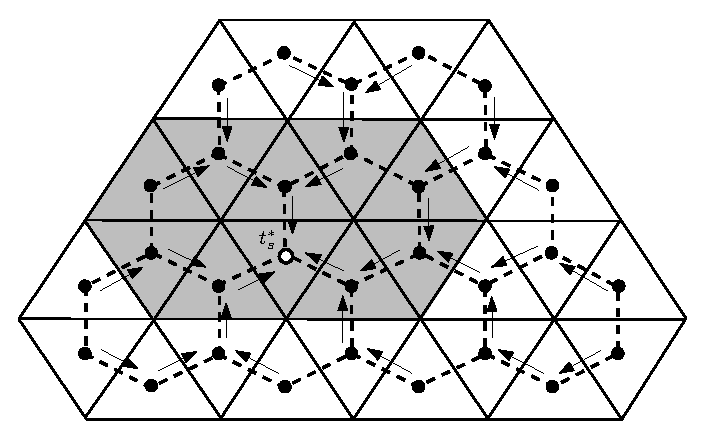
\includegraphics[width=0.6\textwidth]{Fig7}
	  \caption[Dual graph with non-entry edges removed forms a tree]{ 
	    A triangulation is shown with its dual graph. 
	    The arrows indicate the entry edges selected for each triangle when
	    triangle $t_s$ is selected as the root ($\dual{t}_s$ is circled). 
	    The arrows are directed from child to parent.
	    Removing the non-entry edges results in a tree in the dual, rooted at 
	    $\dual{t}_s$.
	    So long as a connected component is convex (e.g., the shaded area) this 
	    tree property holds for the subgraph consisting of only nodes in the
	    component} \label{fig:imp_tree_entry}
  \end{figure}
	  
  \begin{figure}[th]
	  \centering 
	  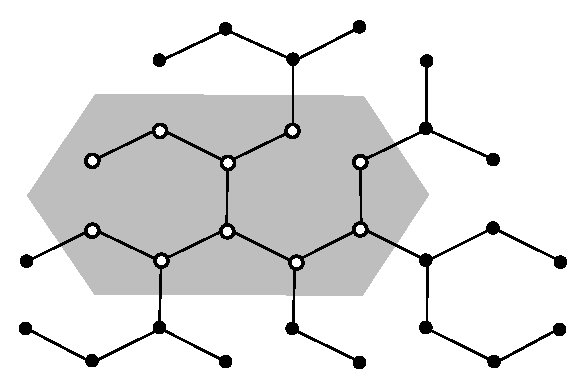
\includegraphics[width=0.6\textwidth]{Fig8}
	  \caption[Tree rooted at $t_s$]{ The tree rooted at $t_s$; hallow
	  nodes indicate red nodes while solid nodes indicate black nodes} \label{fig:implicit_tree}
  \end{figure}

  This result leads to a simple traversal algorithm for connected 
  components, in the case where we know that the region to be reported 
  is convex.
  We summarize with the following lemma.

  \begin{lemma}\label{lem:report_convex_component}
  Let $\triang_C \subset \triang$ be a connected, convex component.
  Given $t_s \in \triang_C$ we can report all triangles in $\triang_C$ with 
  $\BigOh{\frac{|\triang_C|}{\lg{B}}}$ I/Os.
  \end{lemma}

  \begin{proof}
  Performing a depth-first search on a tree on $|\triang_C|$ vertices is equivalent 
  to walking a path of length at most $4 \cdot |\triang_C|$.
  By Theorem \ref{thm:terrain_traversal}, our data structures permit a walk along 
  such a path with a total I/O cost of $\BigOh{ \frac{|\triang_C|}{\lg{B}} }$.

  Let $s$ be some point interior to $\triang_C$, and let $t_s \in \triang_C$ be
  the triangle containing $s$.
  Starting with $t_s$, we implicitly construct a tree in $\dual{\triang}$ using the 
  selection method of~\cite{deberg_et_al_1997}.
  Since $\triang_C$ is convex, removing all subtrees rooted at black nodes results 
  in an implicit tree, rooted at $t_s$, which includes all red nodes in $\triang_C$
  (see Figures \ref{fig:imp_tree_entry} and \ref{fig:implicit_tree}).
  It remains to be proven that the removal of all subtrees rooted at black nodes
  will not result in the removal of any red nodes from the tree.
  Assume that removing the subtree rooted at some black node, $b$ removes some
  red node $r$. 
  Let $q$ be the parent of $b$ in $\triang_C$. 
  The entry edge corresponding to dual edge $(q,b)$ must be on the convex
  hull of $\triang_C$.
  However, this means that $r$ must be outside the convex hull of $\triang_C$, which
  is a contradition. 
  Therefore, no such triangle (node) $r$ can be removed.
  \end{proof}
  
  We give the following corollary to Lemma \ref{lem:report_convex_component}
  with application to rectangular window queries.
  Such queries are a specialization of reporting a convex region 
  and occur commonly in practice.

  \begin{corollary}\label{cor:window_query}
  Given a terrain $\triang$, and a query window $W$, the set of 
  triangles which intersect the query window can be 
  reported with $O \left( \frac{|\triang_W|}{\lg{B}} \right)$ I/Os. 
  \end{corollary}

  \begin{proof}
  The query window problem is equivalent to reporting 
  a connected component where the selection property is that a triangle 
  intersects the query window $W$. 
  The region to be reported is convex, but care must be taken with 
  triangles that intersect the query window boundary. 
  In \cite{deberg_et_al_1997} it is shown that the entry edge selection 
  rule can be modified to disqualify any edge (or portion thereof) that 
  is outside $W$. 
  Using this modification, an implicit rooted tree is still formed on 
  the triangles of $\triang_W$, and we can perform a memoryless 
  depth-first traversal.
  \end{proof}

  % --------------------------------------------------------------------
  \subsubsection{General Connected Components}\label{ssec:gen_con_comp}
  % --------------------------------------------------------------------

  In this section, we present an algorithm that reports connected components 
  that may be non-convex and/or contain holes.
  Using the terminology developed in Section~\ref{ssec:conv_con_comp}, we 
  say $\concomp$ is a connected component in $\triang$, corresponding 
  to $\dual{\concomp}$ in $\dual{\triang}$. 
  Recall that $\dual{\concomp}$ forms a connected component of red nodes 
  in the subgraph formed by all red nodes in $\dual{\triang}$.
  In $\triang$, we can think of the boundary of a connected component being 
  formed by all edges along the outer perimeter of the component
  in addition to any edges along the perimeters of holes. 
  In the dual, the boundary corresponds to the set of edges connecting 
  red vertices in $\dual{\concomp}$, with black vertices in $\dual{\triang}$. 

  In order to report $\concomp$, we select some triangle $s \in \concomp$ as our
  start triangle. 
  We select entry edges relative to an arbitrary point interior to $s$.
  Since $\triang$ itself is convex, we can construct an implicit tree
  on the nodes of $\dual{\triang}$, rooted at $s$.
  We denote this tree $\dual{\triang}_T$.
  
  Let $r$ and $b$ be red and black vertices in
  $\dual{\concomp}$, corresponding to adjacent triangles in $\triang$.
  Let $e$ be the edge of $\triang$ separating triangles $r$ and $b$.
  In $\dual{\triang}$, $e$ corresponds to the edge $(r,b)$.
  While this edge is undirected in $\dual{\triang}$, for the sake of the
  discussion that follows we will assume that in $\dual{\triang}_T$, it
  is directed towards the root, $s$.
  We call such edges \emph{boundary} edges, and classify them according
  to their role in the implicit tree $\dual{\triang}_T$, as follows 
  (see Fig.\ref{fig:imp_tree_non-convex}):
  
  \begin{enumerate}
    \item if $(r,b) \notin \dual{\triang}_T$, then $e$ is a \emph{wall}\footnote{
    All edges on the convex hull of $\triang$ are considered wall edges.} edge, 
    \item if $r$ is the parent of $b$, then $e$ is an \emph{access} edge, and 
    \item if $b$ is the parent of $r$, then $e$ is an \emph{exit} edge.
  \end{enumerate}

  \begin{figure}[th]
	  \centering
		  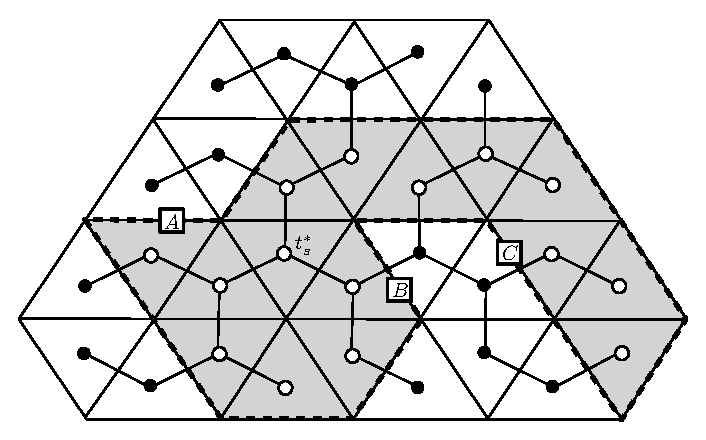
\includegraphics[width=0.6\textwidth]{Fig9}
	  \caption[Boundary edge definitions]{A triangulation and the implicit tree 
	  formed by the entry edges selected for the circled vertex $\dual{t}_s$. 
	  In this case, the connected component of $t_s$ is non-convex so that the tree 
	  formed by only red (hallow) nodes is disconnected. 
	  The boundary edges of the triangulation are indicated by the heavy dashed 
	  line. 
	  Using our notation for boundary edges, A is a \emph{wall} edge, B is an 
	  \emph{access} edge where the tree enters the component, and C is an 
	  \emph{exit} edge where the tree leaves the component}
	  \label{fig:imp_tree_non-convex}
  \end{figure}

  We report the triangles in $\concomp$ using the algorithm 
  $\funccase{DepthFirstTraversal}$ listed in Fig. \ref{fig:traverse_graph_algorithm}.
  The algorithm performs a standard depth-first traversal in 
  $\dual{\triang}_T$, with one important modification. 
  If a branch of the algorithm's execution terminates at an access boundary 
  edge, then the function $\funccase{ScanBoundary}$ (Fig. \ref{fig:scanhandrail_alg}) 
  is invoked. 
  $\funccase{ScanBoundary}$ traverses the chain of boundary edges, and recursively calls 
  $\funccase{DepthFirstSearch}$ at each exit edge. 
  A search structure, $\mathcal{V}$, is maintained to ensure that no boundary edge is 
  scanned more than once.  
  Whenever an access edge is visited during the $\funccase{ScanBoundary}$ 
  or $\funccase{DepthFirstSearch}$ 
  processes, it is added to the search structure $\mathcal{V}$ if it is not already 
  present. 
  If an access edge is encountered that is already in $\mathcal{V}$, then execution 
  of $\funccase{ScanBoundary}$ is halted. 
  Likewise, when $\funccase{DepthFirstTraversal}$ encounters an access edge already in 
  $\mathcal{V}$, it does not invoke $\funccase{ScanBoundary}$. 

  \begin{figure}[h]
  \protect \framebox[0.95\linewidth]
  {
  \begin{minipage}{0.90\linewidth}

  \textbf{Algorithm $\textsc{\funccase{DepthFirstTraversal}}(t_s,s)$} \\
  1. \hspace{3pt} $t \leftarrow t_s$ \\
  2. \hspace{3pt} \textbf{do} \\
  3. \hspace{18pt} \textbf{if}($t$ has unvisited children) \\
  4. \hspace{33pt} $c \leftarrow $ next unvisited child of $t$ \\
  5. \hspace{33pt} \textbf{if}($\mathcal{P}(c) \ne \mathcal{P}(t)$) \\
  6. \hspace{48pt} $e \leftarrow$ boundary edge corresponding to $(c,t)$ \\
  7. \hspace{48pt} \textbf{if}($e$ is an access edge \textbf{and} $e \notin \mathcal{V}$) \\
  8. \hspace{63pt} $\funccase{ScanBoundary(e, t)}$ \\
  9. \hspace{48pt} \textbf{endif} \\
  10. \hspace{30pt} \textbf{else} \\
  11. \hspace{45pt} $t \leftarrow c$ \\
  12. \hspace{30pt} \textbf{endif} \\
  13. \hspace{15pt} \textbf{else} \\
  14. \hspace{30pt} $t \leftarrow$ parent of $t$ \\
  15. \hspace{15pt} \textbf{endif} \\
  16. \textbf{until}($t$ has no more unvisited children \textbf{and} $t=t_s$) \\
  \end{minipage}
  }
  \caption{Algorithm $\funccase{DepthFirstTraversal}$ }
  \label{fig:traverse_graph_algorithm}
  \end{figure}

  \begin{figure}[h]
  \protect \framebox[0.95\linewidth]
  {
  \begin{minipage}{0.90\linewidth}

  \textbf{Algorithm $\textsc{\funccase{ScanBoundary}}(e,t,s)$} \\
  1. \hspace{3pt} $e' \leftarrow$ next boundary edge in counterclockwise direction from $e$ \\
  2. \hspace{3pt} \textbf{do} \\
  3. \hspace{18pt} \textbf{if}($e'$ is an access edge) \\
  4. \hspace{33pt} \textbf{if}($e' \in \mathcal{V}$) \\
  5. \hspace{48pt} \textbf{break} \\
  6. \hspace{33pt} \textbf{else} \\
  7. \hspace{48pt} add $e'$ to $\mathcal{V}$ \\
  8. \hspace{33pt} \textbf{endif} \\
  9. \hspace{18pt} \textbf{endif} \\
  10. \hspace{15pt} \textbf{if}($e'$ is an exit edge) \\
  11. \hspace{30pt} select triangle $t$ adjacent to $e'$ \\
  12. \hspace{30pt} $\funccase{DepthFirstTraversal(t,s)}$ \\
  13. \hspace{15pt} \textbf{endif} \\
  14. \textbf{until}(e' == e) \\
  \end{minipage}
  }
  \caption{Algorithm $\funccase{ScanBoundary}$ }
  \label{fig:scanhandrail_alg}
  \end{figure}

  \begin{lemma}\label{lem:cc_holes_alg_correctness}
  Given a triangle $t_s \in \concomp$, the algorithms 
  $\funccase{DepthFirstTraversal}$ and $\funccase{ScanBoundary}$ report all
  triangles in $\concomp$.
  \end{lemma}

  \begin{proof}
  Let $s$ be the start triangle selected for $\funccase{DepthFirstTraversal}$,
  and let $t \in \concomp$ be a node in $\dual{\triang}$ not reported by 
  $\funccase{DepthFirstTraversal}$.
  Since $s$ is the root of $\dual{\triang}_T$, there is a path connecting $s$ 
  to $t$ in  $\dual{\triang}_T$. 
  If all nodes on the path from $s$ to $t$ in $\dual{\triang}_T$ are red, then
  clearly $\funccase{DepthFirstTraversal}$ reports $t$.
  Thus, there must be black nodes on the path $s \leadsto t$, corresponding to
  the path leaving $\concomp$.
  Let $w$ and $u$ be the first, and last, nodes encountered on the first such
  black subpath on $s \leadsto t$ (it may be the case that $w = u$).
  Let $w'$ be the red node preceeding $w$ on $s \leadsto t$, and let $u'$ be
  the red node following $u$ on the same path (see 
  Figure~\ref{fig:component_subpaths}).
  The edge $(w'w)$ is an exit edge, while $(u,u')$ is an access edge under
  our definitions. 
  The subpath $s \leadsto w'$ is wholly contained in $\concomp$, thus the call
  to $\funccase{DepthFirstTraversal}$ from $s$ reaches $w'$.
  If the access edge corresponding to $(w',w)$ has not 
  been previously visited the $\funccase{ScanBoundary}$ algorithm is invoked.
  The call to $\funccase{ScanBoundary}$ visits the edge $(u,u')$, unless it
  is blocked when it encounters a previously visisted access edge in 
  $\mathcal{V}$.
  This may  occur if one of the recursive 
  calls to $\funccase{DepthFirstSearch}$ made at exit edges during 
  $\funccase{ScanBoundary}$ 
  encounters the same boundary. 
  However, if $\funccase{ScanBoundary}$ is blocked from visiting $(u,u')$ in 
  such a fashion, then $\funccase{ScanBoundary}$ must have been called
  from the blocking access edge. 
  Let $s_0, s_1, \ldots, s_i$ be a sequence of such blocking calls to 
  $\funccase{ScanBoundary}$ along the boundary chain between $(w',w)$ 
  and $(u,u')$. 
  Clearly, the last such call, $s_i$ will result in $(u,u')$ being visited. 
  This same argument can be applied to any other subpaths leaving 
  $\concomp$ on $s \leadsto t$, and as such $\dual{t}$ is visited by 
  $\funccase{DepthFirstTraversal}$.
  \end{proof}

  \begin{figure}[th]
	  \centering
		  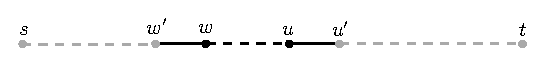
\includegraphics[width=0.6\textwidth]{Fig12}
	  \caption[General component subpaths]{The path through the tree 
	  $\dual{\triang}_T$ connecting nodes $s$ and $t$, which are both
	  part of the connected component $\concomp$. 
	  The path leaves $\concomp$ at $(w',w)$ and re-enters at $(u,u')$}
	  \label{fig:component_subpaths}
  \end{figure}
  
  The I/O cost of reporting a general connected component includes
  the cost to walk the triangles of $\concomp$, plus the cost
  of walking the boundary of $\concomp$.
  We denote by $h$ the size of the boundary, and summarize our I/O
  costs with the following lemma.

  \begin{lemma}\label{lem:io_eff_ccomp}
  The algorithm $\funccase{DepthFirstTraversal}$ reports a connected 
  component 
  $\concomp$ with $h$ boundary edges using 
  $O\left( \frac{|\concomp|}{\lg{\succblksize}} \right) + O(h \log_{B}{h})$ I/Os.
  \end{lemma} 

  \begin{proof}
  Performing depth-first traversal is equivalent to a walk of 
  length at most $4|\concomp|$, which can be performed in 
  $O\left( \frac{|\concomp|}{\lg{\succblksize}} \right)$ I/Os. 
  We must also account for the length of the paths traversed by calls 
  to $\funccase{ScanBoundary}$. 
  Any triangle in $\concomp$ may be visited at most three times, since 
  it may be adjacent to no more than three different boundary chains. 
  Thus, the total additional length of the walks associated with calls 
  to $\funccase{ScanBoundary}$ is bounded by $3|\concomp|$, which 
  increases the length of the path traversed by a constant factor. 

  We must also account for the number of I/Os required to maintain 
  and query the boundary edge structure $\mathcal{V}$. 
  There are $h$ boundary edges, and in the worst case most of these 
  edges may be access edges. 
  Using a B-tree to store $\mathcal{V}$ 
  supports insertions and queries in $O(\log_B{h})$ time.  
  An access edge is added to $\mathcal{V}$ only once, and is visited at 
  most one additional time. 
  Thus the total cost to maintain and query $\mathcal{V}$ is $O(h \log_B{h})$.  
  \end{proof}

  Finally, we account for the space used to store $\mathcal{V}$. 
  Since our triangulation does not store edges, we must have some
  way of uniquely identifying the edges in $\mathcal{V}$.
  We do so by storing the coordinates of the midpoint of each edge, which
  serves as our search key.
  For $\mathcal{V}$ we use a B-tree, and for each edge store a $\bitsPerPoint$-bit 
  key plus a $\lg{N}$ bit pointer. 
  Thus the space for this structure is $\OhOf{h \cdot(\bitsPerPoint + \lg{N})}$ 
  bits. 
  In theory, the size of this structure could be as large as $\concomp$,
  but in many scenarios it will be significantly smaller.  
  The following theorem summarizes our results 
  for convex and general connected components. 
  The space bound adds the space for $\mathcal{V}$ to the bound from
  Theorem \ref{thm:terrain_traversal}.
  The I/O bounds are obtained from Lemmas \ref{lem:report_convex_component} 
  and \ref{lem:io_eff_ccomp}.

  \begin{theorem}\label{thm:conn_comp}
  A triangulation $T$, with $\bitsPerKey$-bit keys per triangle, may be 
  stored using 
  $N(\bitsPerPoint + \bitsPerKey) + O(N) + o(N(\bitsPerPoint + \bitsPerKey)$ 
  bits such that a 
  connected component $\concomp$ may be reported using 
  $O \left( \frac{|\concomp|}{\lg{B}} \right)$ I/Os if $\concomp$
  is convex.  
  If $\concomp$ may be non-convex or have holes, then the query requires 
  $O\left( \frac{|\concomp|}{\lg{B}}  + h \log_B{h}\right)$ 
  I/Os, plus an additional $\OhOf{h \cdot(\bitsPerPoint + \lg{N})}$ bits of storage, 
  where $h$ is the number of boundary edges of 
  $\concomp$.
  \end{theorem}

  % ----------------------------------------------------------------------
  \subsection{Connected Components Without Additional Storage}
  \label{ssec:no_add_storage}
  % ----------------------------------------------------------------------

  One drawback with our technique for reporting connected components 
  in Section~\ref{ssec:gen_con_comp} is that 
  we must store the search structure $\mathcal{V}$ in order to complete the 
  traversal. 
  In this section, we present a revised version of the algorithm that removes 
  the need for this additional data structure, at the cost of performing 
  additional I/O operations.

  Our technique is based on the algorithm of Bose and 
  Morin~\cite{DBLP:conf/isaac/BoseM00}, for the more general case of subdivision 
  traversal in planar subdivisions. 
  That paper, in turn, is a refinement of the algorithm presented by 
  de~Berg~\etal~\cite{deberg_et_al_1997}. 
  The strategy in both papers is to identify a single entry edge on each face. 
  When an edge is visited while reporting the edges of a face, a check is made 
  to determine if it is the (unique) entry edge for an adjacent face. 
  If the edge proves to be an entry edge, then the adjacent face is entered. 
  The resulting traversal is a depth-first traversal of the faces of the 
  subdivision. 
  In both papers, (\cite{DBLP:conf/isaac/BoseM00} and \cite{deberg_et_al_1997}),
  the subdivision is assumed 
  to be represented as a doubly-connected edge list, or a similar 
  topological structure. 

  Bose and Morin~\cite{DBLP:conf/isaac/BoseM00} select entry edges based 
  on a total order $\preceq_p$ on the edges of the subdivision. 
  The position of each edge, $e$ in $\preceq_p$, is determined based on 
  the edge's key. 
  The key is a 4-tuple of properties that can be calculated locally for 
  each edge, based on the edge's geometry. 
  As with our previous entry edge seletion rule, the keys are calculated 
  with repect to a known point interior to the start triangle.
  To determine if an edge is the entry point of a face, the following 
  \emph{both-ways} search is performed.
  Starting at edge $e$, the face is scanned in both directions 
  until either (a) an edge $e'$ is encountered with 
  a lower key than $e$ in $\preceq_p$, or (b) the scans meet without 
  having found any such edge.  
  In case (b), the edge $e$ is then selected as the entry edge for 
  the face.

  The main result of Bose and Morin is that for a subdivision 
  with $N$ vertices, all faces (including edges and vertices) can be 
  reported in $\OhOf{N \log{N}}$ steps. 
  Their approach can also be applied to reporting a connected 
  component of the subdivision in $\OhOf{h \log{h}}$ time, where the 
  $h$ is the number of vertices in the component.  

  In the case presented in this section, we are dealing with 
  triangular faces, so the entry edge can be found in constant time.
  Where the 'search both ways' technique proves useful in our setting 
  is in dealing with the boundary of the component. 
  A hole may consist of 
  one or many faces (triangles), but we treat a hole as if it were a 
  single face.
  For each hole, we want to identify a unique entry edge from among
  the access edges on its boundary.
  Since edges are not explicity stored in our construction, walking
  the boundary involves walking the set of triangles that touch the boundary. 
  This includes all triangles in $\concomp$ that:
  
  \begin{enumerate}
  \item have an edge on the boundary, or
  \item have an adjacent vertex, $p \in P$, that lies on the boundary.
  \end{enumerate}
  
  Let $h'$ denote the number of triangles touching the boundary of
  $\concomp$. 
  This includes both holes in $\concomp$ and its outer boundary.
  A triangle can be adjacent to the boundary at no more than three 
  points (or edges), therefore $h' = \OhOf{|\concomp|}$. 
  
  Assume $H$ is some hole in our component. 
  In order to apply the analysis of Bose and Morin directly to our results, 
  we conceptually add zero length
  \emph{pseudo-edges} to $H$ at any point on the boundary of $H$ that 
  is adjacent to a triangle $t$ which touches $H$ at a point, but which 
  does not share an edge with $H$ (see Fig. \ref{fig:pseudo-face} ). 
  With respect to the key values in $\preceq_p$, we set the value of 
  a key for a pseudo-edge to $\infty$. 
  Since the entry edge in any hole is the edge of minimum key value, 
  no pseudo-edge will ever be selected. 
  Given this definition of a pseudo-edge, the value $h'$ can also 
  be considered the sum of real and pseudo-edges over all holes 
  and the exterior boundary of the component $\concomp$.

  \begin{figure}[th]
	  \centering
		  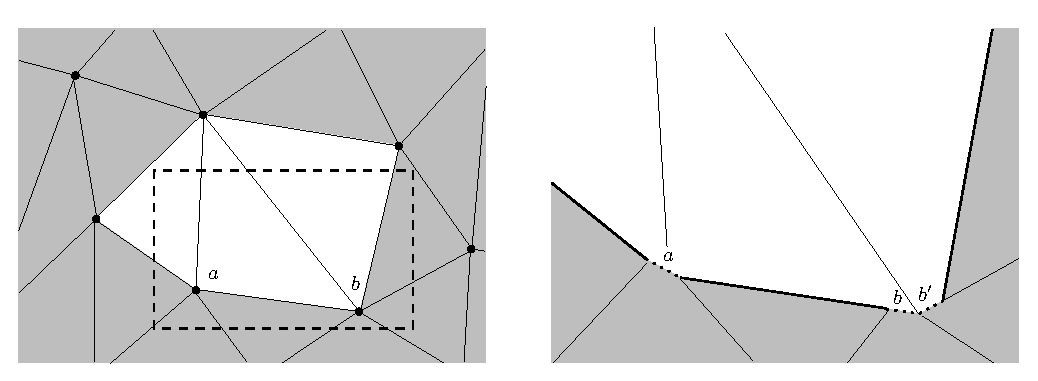
\includegraphics[width=0.8\textwidth]{Fig13}
	  \caption[Psuedo-edges in region boundaries]{The figure on the left 
    shows a portion of a component (grey) with a hole (white). 
	  The dashed box indicates the detailed area shown in the figure on the
	  right. 
	  The right-hand figure shows conceptually how additional edges are 
	  added to the hole boundary, corresponding to triangles in the component.
	  At the point marked $a$, a single pseudo-edge is added as there is 
	  only one non-edge adjacent triangle adjacent to this point. 
	  The point $b$ has two non-edge adjacent triangles, therefore two pseudo-edges 
	  $b$ and $b'$ are added to the hole boundary }
	  \label{fig:pseudo-face}
  \end{figure}

  The following lemma summarizes results for Bose and Morin that can now be 
  applied directly to our setting.

  \begin{lemma}\label{lem:bose_morin_time}
  For a connected component $\concomp$ requiring $h'$ triangles to be visited 
  in order to walk the boundary of all holes plus the exterior boundary of 
  $\concomp$, the both-ways search technique can find entry edges for all 
  holes (and the perimeter) in at most $\OhOf{h' \log{h'}}$ steps, 
  or $\OhOf{h' \log_{\succblksize}{h'}}$ I/Os. 
  \end{lemma}

  \begin{proof}
  Theorem 1 in Bose and Morin \cite{DBLP:conf/isaac/BoseM00} states that 
  a planar subdivision of faces with $n$ vertices can be traversed in 
  $\OhOf{n \log{n}}$ time. 
  By adding zero-length pseudo-edges, we effectively make 
  the set of holes and the exterior boundary equivalent to faces with 
  a total of $h'$ edges. 
  Thus, using the both-ways search, we can locate entry edges with 
  $\OhOf{h' \log{h'}}$ steps. 
  Since we can travel $\OhOf{\log{\succblksize}}$ steps during such 
  searches before incurring an I/O, we can perform all such searches in 
  $\OhOf{h' \log_{\succblksize}{h'}}$ I/Os.
  \end{proof}

  Applying the both-ways search technique presented above requires only 
  minor modifications to our algorithms. 
  In the $DepthFirstTraversal$ algorithm (Fig. 
  \ref{fig:traverse_graph_algorithm}) at line 7 rather than check 
  if $e \in \mathcal{V}$, we perform the both-ways search to determine 
  if $e$ is the unique entry edge. 
  If this is true, we then perform $ScanBoundary$ starting with $e$. 
  The only alteration to the $ScanBoundary$ algorithm 
  (Fig. \ref{fig:scanhandrail_alg}) is that we can omit steps 3 
  through 9, since following the both-ways search we know that $e$ 
  is the  unique entry edge for the boundary or hole.  

  To summarize we have the following theorem.

  \begin{theorem}\label{thm:conn_comp_without_add_storage}
  A triangulation $\triang$, with $\bitsPerKey$-bit keys per triangle, 
  may be stored using $N\bitsPerKey + O(N) + o(N\bitsPerKey)$ bits such 
  that a connected component $\concomp$ may be reported using 
  $\BigOh{\frac{|\concomp|}{\lg{B}} + h' \log_B{h'}}$ I/Os, where 
  $h'$ is the total number of triangles that touch all holes in, 
  plus the boundary of, $\concomp$.
  \end{theorem}





\begin{acknowledgements}
The authors wish to thank the School of Computer Science, Carleton University 
and the Natural Sciences and Engineering Research Council of Canada for financial 
assistance.
The work was done while the second author was at the
School of Computer Science, Carleton University, Canada.
\end{acknowledgements}

% BibTeX users please use one of
%\bibliographystyle{spbasic}      % basic style, author-year citations
\bibliographystyle{spmpsci}      % mathematics and physical sciences
%\bibliographystyle{spphys}       % APS-like style for physics
\bibliography{literature}   % name your BibTeX data base

% Non-BibTeX users please use
%\begin{thebibliography}{}
%
% and use \bibitem to create references. Consult the Instructions
% for authors for reference list style.
%
%\bibitem{RefJ}
% Format for Journal Reference
%Author, Article title, Journal, Volume, page numbers (year)
% Format for books
%\bibitem{RefB}
%Author, Book title, page numbers. Publisher, place (year)
% etc
%\end{thebibliography}

\end{document}
% end of file template.tex

